%=====================================================================
%  PS 647 — Group Project
%  Digital Financial Infrastructure and Financial Inclusion in India
%
%  COMPILER: pdfLaTeX  (Overleaf default — do not switch to XeLaTeX)
%  BIBLIOGRAPHY: BibTeX + natbib  (NOT biber/biblatex)
%
%  On Overleaf: upload this folder as a .zip, set main.tex as the main
%  document, Compiler = pdfLaTeX. Nothing else needs configuring.
%
%  TO HIDE ALL "TO BE COMPLETED" MARKERS BEFORE SUBMISSION:
%      change   \usepackage[...]{todonotes}
%      to       \usepackage[disable]{todonotes}
%  (one line, marked below)
%=====================================================================
\documentclass[11pt,a4paper,oneside]{report}

%--------------------------------------------------- encoding & fonts
\usepackage[T1]{fontenc}
\usepackage[utf8]{inputenc}
\usepackage{lmodern}
\usepackage{microtype}

%--------------------------------------------------- page geometry
\usepackage[a4paper,left=3cm,right=2.5cm,top=2.5cm,bottom=2.5cm]{geometry}
\usepackage{setspace}
\singlespacing

%--------------------------------------------------- maths
\usepackage{amsmath}
\usepackage{amssymb}

%--------------------------------------------------- tables
\usepackage{booktabs}
\usepackage{tabularx}
\usepackage{longtable}
\usepackage{threeparttable}
\usepackage{multirow}
\usepackage{array}
\usepackage{pdflscape}

%--------------------------------------------------- figures
\usepackage{graphicx}
\graphicspath{{images/}}
\usepackage{float}
\usepackage{caption}
\usepackage{subcaption}
\captionsetup{font=small,labelfont=bf}

%--------------------------------------------------- lists, colour, boxes
\usepackage{enumitem}
\usepackage{xcolor}
\definecolor{shadecolour}{RGB}{243,243,240}
\definecolor{rulecolour}{RGB}{120,120,120}
\definecolor{linkcolour}{RGB}{20,60,120}

%--------------------------------------------------- quotes
\usepackage{csquotes}

%--------------------------------------------------- bibliography
\usepackage{natbib}
\bibliographystyle{plainnat}
\setcitestyle{authoryear,round}

%--------------------------------------------------- TODO / stub markers
% >>> CHANGE THE OPTION TO [disable] TO HIDE EVERY STUB MARKER <<<
\usepackage[colorinlistoftodos,textsize=footnotesize,textwidth=2.4cm]{todonotes}

%--------------------------------------------------- hyperlinks (load late)
\usepackage[hidelinks]{hyperref}
\hypersetup{
  colorlinks=true,
  linkcolor=linkcolour,
  citecolor=linkcolour,
  urlcolor=linkcolour,
  pdftitle={Digital Financial Infrastructure and Financial Inclusion in India},
  pdfsubject={PS 647 Group Project},
}
\usepackage{url}
\urlstyle{same}

%=====================================================================
%  PROJECT-SPECIFIC MACROS
%=====================================================================

% The rupee glyph U+20B9 does NOT exist in the T1 font encoding and will
% break a pdfLaTeX build. Always use \rs — never paste the symbol.
\newcommand{\rs}{Rs.\,}

% Marks a section that is deliberately incomplete.
\newcommand{\stub}[1]{%
  \todo[inline,color=yellow!30,caption={TO BE COMPLETED}]{\textbf{To be completed:} #1}}

% Inline emphasis for a pre-committed / pre-registered choice.
\newcommand{\prereg}[1]{\textcolor{linkcolour}{\textbf{#1}}}

% A framed box for material that must not be paraphrased away
% (the pre-committed decision rule, the honest headline).
\newenvironment{keybox}[1]%
  {\begin{center}\begin{minipage}{0.93\textwidth}%
   \vspace{2pt}\color{rulecolour}\hrule\vspace{6pt}%
   \color{black}\textbf{#1}\par\vspace{4pt}\small}%
  {\vspace{6pt}\color{rulecolour}\hrule\vspace{2pt}%
   \end{minipage}\end{center}\vspace{6pt}}

% Shorthand for the two panels, used constantly in Chapter 3.
\newcommand{\panelA}{FY2018--FY2023}
\newcommand{\panelB}{FY2012--FY2023}

% Consistent notation for the three dependent constructs.
\newcommand{\Access}{\textit{Access}}
\newcommand{\Usage}{\textit{Usage}}
\newcommand{\AUG}{\textit{AUG}}

%=====================================================================
\begin{document}

%---------------------------------------------------------- TITLE PAGE
\begin{titlepage}
\centering
\vspace*{2cm}

{\Large\scshape PS 647 --- Group Project\par}
\vspace{1.2cm}

{\color{rulecolour}\rule{\textwidth}{0.4pt}}
\vspace{0.8cm}

{\Huge\bfseries Digital Financial Infrastructure\\[0.25cm]
and Financial Inclusion in India\par}
\vspace{0.6cm}

{\large\itshape A state-level panel study of the access--usage gap\par}
\vspace{0.8cm}

{\color{rulecolour}\rule{\textwidth}{0.4pt}}
\vspace{1.8cm}

% ---------------------------------------------------------------
% EDIT THIS BLOCK: author names, roll numbers, institution, course.
% ---------------------------------------------------------------
{\large
\begin{tabular}{c}
\textbf{Author One} \\ \textit{Roll No. XXXXXXX} \\[0.8em]
\textbf{Author Two} \\ \textit{Roll No. XXXXXXX} \\[0.8em]
\textbf{Author Three} \\ \textit{Roll No. XXXXXXX} \\
\end{tabular}\par}
\vspace{1.8cm}

{\large Department of [Department Name]\par}
{\large [Institution Name]\par}
\vspace{0.6cm}
{\large Course instructor: [Instructor Name]\par}

\vfill
{\large \today\par}
\end{titlepage}

%---------------------------------------------------------- FRONT MATTER
\pagenumbering{roman}

\chapter*{Abstract}
\addcontentsline{toc}{chapter}{Abstract}

India presents a paradox. Adult account ownership rose from 35 per cent in 2011 to roughly 89 per
cent by 2025, yet India records the largest share of \emph{inactive} accounts in the world: about
35 per cent of Indian adults who hold an account hold a dormant one, some seven times the average
across other developing economies \citep{findex2021,findex2025}. Accounts have been opened far
faster than they have been used. This report asks whether the expansion of financial infrastructure
is itself part of that story --- whether expansion has been formal rather than functional.

We build verified state-level panels from nine sources: eight Reserve Bank of India and Government
of India series covering branches, ATMs, deposit and credit account counts, deposit and credit
balances, per-capita state income and adult population, plus state-level digital payment data from
PhonePe Pulse. All-India aggregates reconcile to published figures to within 0.001 per cent.
Hypothesis~1 --- that infrastructure raises \Access{} more than \Usage{} --- is tested on three
tracks by two-way fixed-effects regressions of \Access{}, \Usage{} and their difference, with
standard errors clustered by state. The decision rule for accepting or rejecting it was fixed in
writing before any coefficient was estimated.

On the two \textbf{physical} tracks --- 33 states over \panelA{} and 32 over \panelB{} ---
\textbf{the hypothesis is not supported, and the null is uninformative}. A diagnostic run before
estimation, with thresholds fixed in advance, found that only 7.0 per cent of the variation in
branches per lakh adults and 8.7 per cent of that in ATMs occurs \emph{within} states; roughly 93
per cent is cross-sectional, which is exactly what fixed effects discard. A Hausman test then
rejects random effects decisively, ruling out the estimator that would recover that variation. The
fragility this implies is demonstrated rather than asserted: dropping two observations out of 198
reverses the sign of every ATM coefficient.

On the \textbf{digital} track --- 33 states over FY2019--FY2023, adding UPI adoption --- the
identification problem disappears. Within-state variation in UPI users per adult is 67.1 per cent,
and explanatory power rises from a within-$R^2$ of 0.069 to 0.609 for \Access{}. UPI adoption
raises \Access{} ($+0.439$) more than \Usage{} ($+0.183$), and the gap is significant
($p = 0.020$) --- the first time in this study the access--usage gap is distinguishable from zero.
Decomposing the outcome shows the effect runs \emph{entirely through credit accounts, not deposit
accounts}, which is the reverse of what an accounting artefact would produce, since deposit
accounts are the component definitionally entangled with UPI registration. The result survives
dropping any single state.

Two caveats bound this. The pre-committed hypothesis named branches and ATMs and it failed; UPI was
added \emph{after} seeing that null, so the digital result is exploratory by construction --- a
hypothesis generated by this data, not one tested and passed. And while the identification problem
is solved, the causal one is not: fixed effects do not remove state-specific time-varying
confounders.

\vspace{0.8em}
\noindent\textbf{Keywords:} financial inclusion; access--usage gap; banking infrastructure; digital
payments; UPI; panel data; two-way fixed effects; India; pre-registration.


\tableofcontents
\listoftables

\cleardoublepage
\pagenumbering{arabic}

%---------------------------------------------------------- BODY
\chapter{Introduction, Background and Literature}
\label{ch:intro}

\section{The puzzle}
\label{sec:puzzle}

Between 2011 and 2017 the share of Indian adults holding a bank account rose from 35 to 80 per
cent \citep{findex2021}, reaching roughly 89 per cent by the 2025 Global Findex round
\citep{findex2025}. Much of that movement came from a single programme: the Pradhan Mantri Jan Dhan
Yojana (PMJDY), launched in August 2014, under which more than 56 crore accounts had been opened by
August 2025 \citep{pmjdy2025}. Measured by the indicator that dominates international league
tables, India solved financial exclusion inside a decade.

The same surveys record a second fact that sits uncomfortably beside the first. India has the
largest share of \emph{inactive} accounts of any country measured: roughly 35 per cent of Indian
adults who own an account report that it is dormant, some seven times the 5 per cent average across
other developing economies \citep{findex2021}. Official figures point the same way --- about 26 per
cent of PMJDY accounts, some 15 crore, are reported inoperative, with an average balance of roughly
\rs 4,808 \citep{pmjdy2025}. Among adults holding a dormant account, 49 per cent cite distance to
the institution and 46 per cent say they did not need an account \citep{findex2021}.

An account that exists but is never used counts as inclusion in every headline statistic while
delivering none of the consumption-smoothing, risk-pooling, or credit benefits that justify the
policy effort. The gap between \emph{having} an account and \emph{using} one is the central
empirical object of this report, and we refer to it throughout as the \textbf{access--usage gap}.

The gap could arise from low incomes, informality, distrust, poor financial literacy, or the simple
fact that many accounts were opened to receive a one-off transfer. This report examines a candidate
that policy can actually move: the infrastructure through which banking is delivered. The reasoning
is asymmetric in an important way. Opening an account is largely a \emph{supply-side} decision ---
banks can be given targets and audited against them, and Indian branch licensing has been used this
way since the 1970s. Using an account is a \emph{demand-side} decision shaped by income,
informality, and trust. Infrastructure relaxes the first constraint directly; whether it relaxes
the second is an empirical question. If the asymmetry is real, expanding infrastructure should raise
measured access more than measured usage, and the gap should \emph{widen} as infrastructure
expands. Expansion would be, in a phrase used throughout, \textbf{formal rather than functional}.

\section{Background}
\label{sec:background}

Three policy waves have shaped Indian financial inclusion, and this study's sample period sits
inside the third. Following bank nationalisation in 1969, the RBI operated a licensing rule under
which a bank could open a branch in an already-banked location only if it also opened four in
unbanked ones \citep{burgess2005}; the resulting 1977--1990 expansion remains the most studied
episode in the Indian financial-development literature. From the mid-2000s financial inclusion
became an explicit objective, bringing the no-frills account, the business correspondent model, and
the Rangarajan Committee report \citep{rangarajan2008}, together with measurement frameworks
\citep{sarma2008,sarma2012}. From 2014, PMJDY drove ownership toward saturation while the
technology stack sometimes called ``India Stack'' --- biometric identity, interoperable real-time
payments, and consented data sharing --- rewired how retail payments are made \citep{dsilva2019}.
The Unified Payments Interface processed roughly 83.7 billion transactions in calendar 2023, 131.1
billion in 2024, and 228.3 billion in 2025 \citep{npci2025}. This report's sample window sits almost
exactly on top of that transition, a point taken up in Section~\ref{sec:h1-digital}.

India also measures inclusion officially. The RBI's composite Financial Inclusion Index rose from
64.2 in March 2024 to 67.0 in March 2025 \citep{rbi_fiindex2025}, and is built from three parameters
with fixed weights: \textbf{Access 35 per cent, Usage 45 per cent, Quality 20 per cent}. Two
observations follow. First, the RBI's own scheme weights usage \emph{above} access --- an implicit
acknowledgement that account counts overstate inclusion. Second, those weights exist to collapse
three dimensions into one number, whereas this report does the opposite: it holds Access and Usage
apart precisely so their \emph{difference} can be estimated and tested. The weights are therefore
not applicable here, and Section~\ref{sec:h1-variables} records why applying them would have been
an error rather than a refinement.

\section{Literature}
\label{sec:literature}

\paragraph{Access as a supply-side lever.} The foundational result is \citet{burgess2005}, who
exploit the 1977--1990 licensing rule as policy-driven variation in rural branch openings and find
that branch expansion reduced rural poverty. The paper established both a substantive claim ---
that physical banking infrastructure has real welfare consequences --- and a methodological
template: administrative state panels, with infrastructure variation that is not simply a response
to local prosperity. The broader literature is consistent: \citet{beck2007} find financial
development disproportionately raises the incomes of the poor, and \citet{allen2016} document that
cost and proximity are among the strongest correlates of both ownership and use. One caution
prefigures our own conclusion. \citet{buliskeria2022} revisit \citet{burgess2005} and find the
poverty effect does not survive once additional policy breaks are accounted for. The lesson is not
that branches do not matter, but that in this literature the identifying variation is often thinner
and more fragile than it appears, and claims should be stress-tested against perturbations of the
sample. Chapter~\ref{ch:h1} does exactly that, and the stress test produces its most informative
result.

\paragraph{Access is not usage.} A large experimental literature establishes that removing the
barriers to \emph{opening} an account does not reliably produce \emph{use} of it. The clearest
statement is \citet{dupas2018}, who randomly offered free basic accounts in Uganda, Malawi, and
Chile: over two years only 17, 10, and 3 per cent of treated individuals respectively made five or
more deposits, and intention-to-treat effects on savings were indistinguishable from zero. Their
conclusion is the proposition this report takes to Indian administrative data --- ``policies merely
focused on expanding access to basic accounts are unlikely to improve welfare noticeably on
average.'' \citet{karlan2014} reach a compatible position, finding the binding constraints
frequently behavioural and transactional rather than a matter of account availability. This
report's contribution to the strand is one of scale and setting: the experimental evidence is
individual-level and drawn from three countries, and we ask whether the same wedge is visible in
the administrative aggregates of a country of 1.4 billion people, and whether it responds to the
infrastructure variable Indian policy actually controls.

\paragraph{Measuring inclusion.} How inclusion is measured determines what can be found.
\citet{sarma2008,sarma2012} construct a multidimensional index combining penetration, availability,
and usage; the RBI's FI-Index follows the same logic. Composite indices suit ranking and
monitoring, but they are poorly suited to the question asked here: if access and usage are averaged
into one index, the wedge between them becomes unobservable by construction --- and the wedge is
the object of interest. This report therefore departs from the index tradition deliberately.

\paragraph{Digital payments and the substitution of channels.} The final strand asks whether
physical infrastructure is still the relevant infrastructure. \citet{suri2016} show that expanded
mobile-money access in Kenya produced long-run poverty reductions operating through risk-sharing
and occupational change rather than account ownership as such. \citet{crouzet2023} show how India's
2016 demonetisation triggered durable adoption of electronic payments, shaped by network effects
rather than infrastructure stock. \citet{dsilva2019} argue that the design of India's digital public
infrastructure, rather than the density of physical bank premises, is what changed the cost of a
transaction. These matter for interpretation: if the marginal channel for financial activity
shifted from the branch to the phone during our window, a null result for branches and ATMs may be
a substantive statement about channel substitution rather than a measurement failure.

\paragraph{Where this report sits.} The experimental literature establishes the access--usage wedge
at the individual level but cannot speak to national infrastructure policy; the Indian panel
literature establishes that infrastructure has real effects but treats inclusion as a single
dimension. We combine the two --- an administrative state panel, with access and usage held apart
as separate outcomes --- so that the \emph{differential} effect of infrastructure can be estimated
directly.

\section{Hypotheses}
\label{sec:hypotheses}

The report tests three hypotheses. The first is developed and estimated in full in
Chapter~\ref{ch:h1}; the remaining two are reported in Chapters~\ref{ch:h2} and~\ref{ch:h3}.

\begin{keybox}{Hypothesis 1 (Chapter~\ref{ch:h1})}
Greater financial infrastructure raises financial inclusion, but its effect on \textbf{access} is
stronger than its effect on \textbf{usage}.

\medskip
\emph{Rationale.} Opening an account is a supply-side decision that banks can be pushed to make.
Using an account is a demand-side decision shaped by income, trust, and informality.
Infrastructure removes the first constraint, not the second.

\medskip
\emph{Expected:} $\beta_{\text{access}} > \beta_{\text{usage}} > 0$, with the difference
statistically significant.
\end{keybox}

\stub{State Hypotheses 2 and 3 in the same format --- claim, rationale, expected sign pattern ---
then develop them in Chapters~\ref{ch:h2} and~\ref{ch:h3}.}

\begin{keybox}{Hypothesis 2 (Chapter~\ref{ch:h2})}
\textit{[Statement to be supplied.]}
\end{keybox}

\begin{keybox}{Hypothesis 3 (Chapter~\ref{ch:h3})}
\textit{[Statement to be supplied.]}
\end{keybox}

\section{Contribution and roadmap}
\label{sec:contribution}

This report makes four contributions. \textbf{First}, a verified state-year panel assembled from
nine sources --- eight official series using three different year conventions, three different
state-boundary vintages and two different bank universes, plus state-level digital payment data ---
whose all-India aggregates reproduce published figures to within 0.001 per cent, with no imputation
and no missing cells. \textbf{Second}, a direct test of the access--usage wedge on administrative
data, in which the wedge is estimated as its own equation and therefore carries its own standard
error rather than being inferred by eye from two coefficients. \textbf{Third}, a decision rule
written down with its consequences before any coefficient was computed and never revised, which
proved load-bearing twice over: it delivers the verdict on physical infrastructure, and it is what
forces the honest statement that the digital result --- added after that verdict was known --- is
exploratory rather than a test that was passed. \textbf{Fourth}, a negative result that turns into
a positive one by diagnosis rather than by search. Physical infrastructure stocks move too slowly
within states for a short fixed-effects panel to identify their effect; the same diagnostic that
establishes this identifies digital payment adoption as a measure that does move, and on it the
predicted pattern appears --- running entirely through credit accounts rather than deposit
accounts, which is the reverse of what a mechanical artefact would produce.

\medskip
\noindent
Chapter~\ref{ch:data} documents the panels. Chapter~\ref{ch:h1} develops and tests Hypothesis~1 in
full, on three tracks: two measuring infrastructure physically, and one substituting digital
payment adoption. Chapters~\ref{ch:h2} and~\ref{ch:h3} present the second and third hypotheses, and
Chapter~\ref{ch:conclusion} synthesises across the three and concludes.
Appendix~\ref{app:decisions} reproduces the full decision log.

\chapter{Data and Panel Construction}
\label{ch:data}

This chapter documents the panel the hypothesis chapters draw on. It comes first because the
construction is shared, and because several choices made here --- the year-alignment rule above all
--- silently corrupt results if got wrong and are invisible in the output if got right. Every
choice was logged when it was taken, with its rationale; the log is Appendix~\ref{app:decisions},
and decisions are cited below by identifier (D1, D2, \ldots).

\section{Unit of analysis and coverage}
\label{sec:data-unit}

The unit of observation is the \textbf{state--financial year}, and every variable is a
\textbf{stock as at 31 March}, not a flow. A financial year is identified by the calendar year of
the 31 March on which it closes: \texttt{fy\_end}~$=2018$ denotes the position as at 31 March 2018,
the close of financial year 2017--18.

\begin{table}[H]
\centering
\caption{Panel coverage}
\label{tab:panels}
\small
\begin{tabular}{lccccl}
\toprule
Panel & Window & Years & States & $N$ & Infrastructure measured \\
\midrule
Track 1 & \panelA{} & 6 & 33 & 198 & Branches and ATMs \\
Track 2 & \panelB{} & 12 & 32 & 384 & Branches only \\
Track 3 & FY2019--FY2023 & 5 & 33 & 165 & Branches, ATMs and UPI \\
\bottomrule
\end{tabular}
\end{table}

\noindent
All three panels are \textbf{balanced and complete}: every state appears in every year, with no
missing cells and no non-positive values in any series. The state counts differ for one documented
reason given in Section~\ref{sec:data-harmonisation}. ATMs cannot be extended before 2018, because
RBI's state-wise release begins there, which is why Track~2 carries branches alone; Track~3 starts
at FY2019 because that is the first complete financial year of digital payment data. Track~3's
banking columns are asserted \textbf{identical} to Track~1's, so the earlier results remain
reproducible from an untouched file and the tracks stay directly comparable.

\section{Sources}
\label{sec:data-sources}

Nine series are used. Eight are official publications of the RBI or the Government of India, with
one academic redistribution filling a single year; the ninth is the digital payment series
introduced for Track~3.

\begin{table}[H]
\centering
\caption{Source of each series}
\label{tab:sources}
\scriptsize
\begin{tabularx}{\textwidth}{@{}p{2.7cm}p{3.3cm}Xp{1.7cm}@{}}
\toprule
\textbf{Series} & \textbf{Publication} & \textbf{Table / report} & \textbf{Role} \\
\midrule
Bank branches & RBI \emph{Handbook of Statistics on Indian States}, 2024--25 &
Table 152, bank offices of scheduled commercial banks, end-March & Independent \\
\addlinespace
ATMs & RBI \emph{State-wise and Region-wise Deployment of ATMs} &
Standalone quarterly release; end-March files 2018--2024 & Independent \\
\addlinespace
Deposit accounts & RBI Basic Statistical Returns (BSR-2), via DBIE/CIMS &
Report 853, Annual BSR-2 Table 2.3; 31 March 2018 from India Data Portal & \Access{} \\
\addlinespace
Credit accounts & RBI Basic Statistical Returns (BSR-1), via India Data Portal &
Derived state--year credit accounts 2010--2023, including RRBs & \Access{} \\
\addlinespace
Deposits outstanding & RBI \emph{Handbook} & Table 155, deposits of SCBs (\rs crore) & \Usage{} \\
\addlinespace
Credit outstanding & RBI \emph{Handbook} & Table 156, credit of SCBs (\rs crore) & \Usage{} \\
\addlinespace
Per-capita NSDP & RBI \emph{Handbook} & Table 19, per-capita NSDP, current prices & Control \\
\addlinespace
Adult population & Technical Group on Population Projections (2020) &
Annual totals with quinquennial age structure; 1 March series & Denominator \\
\addlinespace
Digital payments & PhonePe Pulse open data release &
Registered users, transaction count and value, by state and quarter & Independent \\
\bottomrule
\end{tabularx}
\end{table}

\noindent
Retrieval was non-trivial in each case. The Handbook tables \citep{rbi_handbook} are HTML only,
each split across two blocks covering earlier and later years, and were parsed and stitched
programmatically. The ATM release \citep{rbi_atm} is navigable only through an ASP.NET postback
widget rather than plain URLs, so per-release permalinks were harvested by scripting those
postbacks. The BSR returns \citep{rbi_bsr} are no longer published as static files at all --- the
legacy links redirect to a single-page application --- and were retrieved programmatically from the
DBIE/CIMS API; the 31 March 2018 deposit-account figures, which the current report does not reach
back to, come from an academic redistribution of the same returns \citep{idp}. Adult population
derives from the official projections report \citep{popproj2020}.

\section{The year-alignment rule}
\label{sec:data-years}

Three year conventions are in play, and they disagree on labels even when they agree on dates. This
is the easiest place in the project to introduce a silent one-year offset --- an error that
produces no missing value, no warning, and no implausible number, and simply biases every estimate.
The Handbook banking tables and the ATM release label a stock as at 31 March 2018 as
\texttt{2018}; the Handbook NSDP tables call the same financial year \texttt{2017-18}; the
population projections date their stock \texttt{1 March 2018}.

\begin{keybox}{Alignment rule (D5, D9)}
Banking year $Y$ $\;\equiv\;$ NSDP financial year $(Y-1)$--$Y$ $\;\equiv\;$ population at
1 March $Y$.

\medskip
All three are recorded in one canonical column, \texttt{fy\_end}, added to all eight input files.
Merging and filtering use \texttt{fy\_end} only, and it supplies the year fixed effect.
\end{keybox}

\noindent
Of the eight files only the income file required conversion; native labels were retained alongside
\texttt{fy\_end} so the original coding stays auditable. The 1 March population series is used
rather than 1 July or 1 October: every numerator is a stock at 31 March, so the denominator must be
a stock at approximately the same instant --- one month away rather than six. The rule was verified
against published figures rather than assumed, as Section~\ref{sec:data-validation} records.

\section{State harmonisation}
\label{sec:data-harmonisation}

Fixed effects require each unit to denote the same thing in every year. India's boundaries changed
inside both windows and, more awkwardly, different sources record the same change in different
years. Three adjustments follow.

\textbf{Units dropped (D1).} Lakshadweep and the combined Dadra \& Nagar Haveli and Daman \& Diu
are dropped: no per-capita NSDP is published for either in any year, so neither can carry the
income control. Both are very small; the panel goes from 35 units to 33.

\textbf{Units merged (D2).} Jammu \& Kashmir with Ladakh, and Dadra \& Nagar Haveli with Daman and
Diu, \emph{in every year}. Merging only from the year of the formal change fails because the
sources disagree about when that was: in the Handbook, Daman \& Diu goes blank from 2020 exactly as
Dadra \& Nagar Haveli jumps from 59 to 110 branches, whereas the ATM files keep three separate
columns until 2021. Summing all components in all years is the only rule producing a continuous
series in both sources simultaneously.

\textbf{Andhra Pradesh and Telangana, twelve-year panel only (D13).} Telangana was carved out of
Andhra Pradesh in June 2014, so in the twelve-year panel it shows \emph{zero} branches, deposits and
credit for 2012--2014, its activity being recorded inside Andhra Pradesh. Branches confirm the
mechanism exactly: Andhra Pradesh falls from 9,900 in 2014 to 6,290 in 2015 as Telangana appears
with 4,721, and the combined series runs continuously from 9,900 to 11,011. The two are therefore
summed in every year, which is why Track~2 has 32 units. The failure mode is instructive: had the
merge been missed, three state-years would have entered recording zero infrastructure alongside
zero deposits --- outliers positioned precisely to manufacture a spurious \emph{positive}
association between infrastructure and inclusion, the sign the hypothesis predicts. It was caught
by a completeness check flagging zeros, not by inspecting results.

\begin{keybox}{General rule}
Merges are performed on \textbf{raw levels} --- branches, ATMs, deposits, credit, account counts,
population --- \textbf{before} any ratio is computed. Ratios are never averaged across merged units.
\end{keybox}

\noindent
After upper-casing and standardising ``AND'' to ``\&'', 34 of 37 units match exactly across
sources; the exceptions are Delhi, Jammu \& Kashmir, and Daman \& Diu, each named differently in
the population or ATM files. Matching uses \textbf{word boundaries} rather than substrings: a naive
substring test folds \texttt{ANDAMAN} into the Daman group, an error that occurred once during
preparation and is now guarded by an explicit assertion.

\section{Validation}
\label{sec:data-validation}

The panel was checked against independently published aggregates rather than accepted on trust.
All-India ATM totals recomputed from the state columns match RBI's published national figures
exactly in every year 2018--2024 (222,066 in 2018 through 257,654 in 2024; the 2024 decline is
genuine decommissioning, not a parsing error). State-by-year deposit amounts differ from Handbook
Table 155 by a median of 0.0001 per cent, and credit amounts from Table 156 by 0.001 per cent.
Population totals reproduce from the sum of age bands, and the published 18+ figure reproduces from
a residual identity, for all 23 states that print it. On year alignment, Maharashtra at
\texttt{fy\_end}~$=2018$ returns 12,545 branches, 25,651 ATMs and per-capita income of
\rs 172,663 --- all matching RBI's published values exactly, confirming no offset was introduced.
Completeness is asserted in code: 198 and 384 rows, balanced, no nulls, no zeros.

\section{The digital payment series}
\label{sec:data-digital}

Track~3 requires a measure of digital financial infrastructure at state level. India has no
official state-wise UPI release covering the full window, so the series used is PhonePe Pulse
\citep{phonepepulse}, the open data release of one of the two largest UPI applications: registered
users, transaction counts and transaction value, by state and calendar quarter.

Conversion to the panel's year convention follows the same rule as everything else. Transactions
and value are \textbf{flows}, summed over the four quarters making up each financial year;
registered users is a \textbf{stock}, taken at the quarter ending 31 March and verified monotone
across all quarter transitions. Denominators follow the same access/usage distinction as the
banking series: registered users \textbf{per adult}, transactions and value \textbf{per capita}.
Coverage is complete --- 36 raw states across 34 quarters with no gaps and no missing amounts ---
and every one of the 33 panel states is present in every year.

Four independent validations were run rather than taking the release on trust. The transaction-type
split (peer-to-peer, retail, utility) reproduces the aggregate total to \textbf{0.000000 per cent}
across all 1,224 state-quarters, meaning two independently maintained trees within the release
agree exactly. Registered users reach \textbf{45.5 crore} at 31 March 2023, against PhonePe's own
publicly stated figure of over 45 crore. Transactions total \textbf{44.3 billion} in FY2023 against
roughly 84 billion for all of UPI that year \citep{npci2025}, consistent with the firm's
approximately 50 per cent market share. And the implied mean ticket size of \rs 1,593 confirms
amounts are denominated in rupees rather than paise.

Three caveats follow the series into the analysis and are revisited in
Section~\ref{sec:h1-limitations}. \textbf{PhonePe is one firm, not the market}, so this measures
PhonePe penetration as a proxy for digital payment penetration, and because market share varies by
state, cross-state levels are noisier than within-state growth --- which is fortunate, since
within-state growth is what the estimator uses. \textbf{Registered users are accounts, not people},
so one person with two numbers counts twice. And transactions are attributed to the \textbf{user's
registered state}, a third attribution rule alongside the branch-location and place-of-sanction
rules already in the panel.

\section{Known limitations of the data}
\label{sec:data-defects}

Three defects are carried openly rather than silently repaired, and each is revisited where it
bears on results.

\paragraph{A break in RBI's own deposit-account series (D7).} The savings-account column of BSR-2
is discontinuous for three states: Delhi runs 35.5, 38.7, \textbf{106.1}, 130.9, 159.4 million
accounts, breaking from 2023 and persisting; Haryana runs 47.7, 52.6, \textbf{102.1}, breaking from
2024; Chandigarh runs 2.98, \textbf{5.03}, 3.25, spiking in 2023 and reverting. This is an error in
RBI's published source, not in extraction --- the component columns reproduce the published total
exactly wherever both are printed --- and the likely cause is a bank reclassifying savings accounts
to a head-office location. The symptom is visible downstream: deposit accounts per adult reaches
7.99 for Delhi in 2023 and 7.69 for Chandigarh in 2023, against roughly 1 to 3.5 elsewhere. Two of
the four affected cells fall inside \panelA{}. The decision, taken \emph{before} estimation, was to
retain them in the main specification and re-run without them as a robustness check;
Section~\ref{sec:h1-robustness} reports what happened, and it is the most consequential result in
the report. Goa sits at 5.45--5.73 across \emph{all} six years and Chandigarh at 5.1--5.4 outside
2023 --- high but flat, so genuine levels rather than defects.

\paragraph{Adult population is interpolated, not published (D6).} The projections publish annual
totals for 2011--2036 but age structure only at five-year anchors, so there is no published annual
adult count. The 18+ series is \emph{derived}: the adult share is linearly interpolated between
anchors and applied to the published annual total. Totals are official; adult counts are ours. Of
the 266 state-years in the underlying file, 243 rest on an interpolated share. The consequence goes
beyond ordinary measurement error, as Section~\ref{sec:h1-gate} develops: being near-linear, the
series is unusually smooth, and as the denominator of every per-adult ratio it contributes almost no
independent variation --- it deflates a trend without adding movement to it. A further caveat
attaches to a few units: the source excludes Goa from its age-structure exercise and reports the
seven smaller north-eastern states only in combination, so proxy shares were assigned and flagged.

\paragraph{Universe and basis of the credit-account series (D8).} The two halves of \Access{}
initially rested on different bank universes: deposit accounts from BSR-2 \emph{include} regional
rural banks, while the quarterly BSR-1 credit series \emph{excludes} them and records loans by place
of sanction rather than utilisation. Excluding RRBs removes a median of roughly 18 per cent of
credit accounts nationally, but unevenly --- 65 per cent in Mizoram, 39 in Tripura, 33 in Uttar
Pradesh --- and the share drifts within states over time, so state fixed effects do not absorb it.
Critically, it bites hardest in exactly the rural, lower-income states the hypothesis is about. The
series was therefore switched to an RRB-inclusive, place-of-utilisation file covering 2010--2023.
The two could not be reconciled arithmetically --- differencing them produced impossible negative
values for Maharashtra, because they differ on \emph{where} a loan is counted as well as on
\emph{which} banks --- so this is a replacement, not an adjustment. The cost is FY2024, which fixes
\panelA{} at six years; the incidental benefit is that the last missing cell, Gujarat's FY2023--24
income, falls outside the window, leaving the panel perfectly balanced. One asymmetry remains:
deposit accounts are recorded by branch location and credit accounts by place of utilisation, and
neither corresponds to depositor or borrower residence.

\section{What the hypothesis chapters draw from this panel}
\label{sec:data-usage}

Chapter~\ref{ch:h1} uses all nine series: the eight banking and demographic series across all
three tracks, and the digital payment series for Track~3.

\stub{If Hypotheses 2 and 3 use series beyond the eight above, add them to
Table~\ref{tab:sources} and document any extra harmonisation here, so this chapter remains the
single place the panel is described.}

\chapter{Hypothesis 1: Infrastructure and the Access--Usage Gap}
\label{ch:h1}

The hypothesis is tested on three panels, built in the order they appear here. Tracks~1 and~2
measure infrastructure physically, as branches and ATMs; both fail, and
Section~\ref{sec:h1-gate} shows they were always going to. Track~3 substitutes the infrastructure
that actually moved over the sample window --- digital payments --- and recovers the pattern the
hypothesis predicts. The distinction between what was pre-committed and what came afterwards is
load-bearing throughout, and Section~\ref{sec:h1-exploratory} states it plainly rather than
leaving it to a footnote.

\begin{table}[H]
\centering
\caption{The three tracks}
\label{tab:tracks}
\small
\begin{tabular}{@{}llccl@{}}
\toprule
Track & Window & $N$ & Infrastructure measured & Outcome \\
\midrule
1 & \panelA{} & 198 & Branches, ATMs & Fails; cannot be tested \\
2 & \panelB{} & 384 & Branches only & Fails; fragility removed \\
3 & FY2019--FY2023 & 165 & Branches, ATMs, \textbf{UPI} & Predicted pattern recovered \\
\bottomrule
\end{tabular}
\end{table}

\section{Hypothesis and pre-commitment}
\label{sec:h1-hypothesis}

\begin{keybox}{Hypothesis 1}
Greater financial infrastructure raises financial inclusion, but its effect on \textbf{access} is
stronger than its effect on \textbf{usage}.

\medskip
\emph{Rationale.} Opening an account is a supply-side decision that banks can be pushed to make.
Using an account is a demand-side decision shaped by income, trust, and informality.
Infrastructure removes the first constraint, not the second.

\medskip
\emph{Expected:} $\beta_{\text{access}} > \beta_{\text{usage}} > 0$, with the difference
statistically significant.
\end{keybox}

\noindent
The hypothesis is directional twice over: both effects should be \emph{positive}, and the access
effect should be \emph{larger}. Positive and equal effects would reject it while remaining a
substantive result --- genuine deepening rather than formal expansion. Both effects at zero would
be uninformative until the identifying variation had been examined. These readings were tabulated
in advance, and Section~\ref{sec:h1-verdict} returns to that table.

Before any coefficient was estimated, a rule was fixed in writing for what would count as support.

\begin{keybox}{Decision rule, fixed before any result was seen (D10)}
Hypothesis~1 is \textbf{fully supported only if
$\beta_{\text{access}} > \beta_{\text{usage}} > 0$ holds for branches \emph{and} for ATMs}. If it
holds for only one, that is reported as \textbf{partial support}, naming which. This is
pre-committed; it is not to be revised after the coefficients are seen.
\end{keybox}

\noindent
Two features of that rule matter for everything below. It names branches and ATMs specifically ---
UPI is not in it, because UPI was not in the design when it was written. And it was not revised:
the physical verdict reported in Section~\ref{sec:h1-verdict} is the verdict the rule returns.

A second pre-commitment was recorded after the pre-estimation diagnostic failed and before
estimation proceeded: a null result does \textbf{not} license the conclusion ``infrastructure does
not raise access'', being indistinguishable from ``the regressors moved too little to detect an
effect''; any null must be reported with the within-state variation figures attached (D11).

\section{Variables and specification}
\label{sec:h1-variables}

\subsection{Independent variables}

Infrastructure enters in natural units, with no composite index:
\[
\text{Branch}_{it} = \frac{\text{branches}_{it}}{\text{adults}_{it}}\times 10^5,
\qquad
\text{ATM}_{it} = \frac{\text{ATMs}_{it}}{\text{adults}_{it}}\times 10^5,
\qquad
\text{UPI}_{it} = \frac{\text{registered users}_{it}}{\text{adults}_{it}}.
\]

An earlier design combined branches, ATMs and PMJDY accounts into one normalised index. It was
abandoned for three reasons (D3, D10). \textbf{PMJDY had to go, and its removal proved
load-bearing:} PMJDY accounts are an \emph{account count}, so placing them among the regressors
while deposit and credit account counts sit among the outcomes would put an account count on both
sides of the equation, manufacturing exactly the mechanical correlation the design warns against.
\textbf{Separating branches from ATMs is statistically safe:} their raw correlation is 0.904, but
that is almost entirely cross-sectional, and after state and year demeaning --- the variation the
model actually uses --- it falls to 0.305, with a variance inflation factor of 1.10.
\textbf{Separating them makes a prediction an index cannot:} a branch is where an account is
\emph{opened}, an ATM where it is \emph{used}. Abandoning the index also removed two arbitrary
choices, the 0--1 rescaling of the regressors and the branches-versus-ATMs weighting, and left
coefficients in interpretable units.

For Track~3, the digital measure is \textbf{registered UPI users per adult}, in levels. Three
candidates existed. Transactions per capita and value per capita were rejected as regressors
because they are themselves \emph{usage} of the digital channel, and using a flow to explain a flow
of the same kind would be close to circular. Registered users is an adoption stock --- whether the
channel is available and taken up at all --- which is the role branches and ATMs play on the
physical side. Levels rather than logs keeps all three infrastructure regressors in the same kind
of unit (D16).

\subsection{Dependent variables}

Four indicators form two constructs, with denominators the design distinguishes deliberately:
\textbf{access is measured per adult, usage per capita}.

\begin{table}[H]
\centering
\caption{Construction of the dependent variables}
\label{tab:dvconstruction}
\small
\begin{tabular}{@{}lllc@{}}
\toprule
Construct & Indicator & Denominator & Entangled with UPI? \\
\midrule
\multirow{2}{*}{\Access{}}
 & Deposit accounts per adult & Population 18+ & \textbf{Yes} (see \S\ref{sec:h1-decomp}) \\
 & Credit accounts per adult  & Population 18+ & No \\
\addlinespace
\multirow{2}{*}{\Usage{}}
 & Deposits per capita (\rs) & Total population & No \\
 & Credit per capita (\rs)   & Total population & No \\
\bottomrule
\end{tabular}
\end{table}

\noindent
Each indicator is rescaled by pooled min--max normalisation,
$\tilde{x}_{it} = (x_{it} - \min x)/(\max x - \min x)$, with the extremes taken over all
state-years rather than within each year, so that genuine growth over time --- which is what the
fixed-effects model estimates from --- is preserved rather than erased. The constructs are the
simple average of their two components, and the gap is their difference:
$\Access{} = \frac{1}{2}(\tilde{d} + \tilde{c})$,
$\Usage{} = \frac{1}{2}(\tilde{D} + \tilde{C})$,
$\AUG{} = \Access{} - \Usage{}$. The normalisation for Track~3 is held at the Track~1 scaling, so
the dependent variables are identical across tracks and the results stay comparable (D15).

\subsection{Specification}
\label{sec:h1-spec}

Three equations are estimated by two-way fixed effects with standard errors clustered by state.
Writing $\mathbf{X}_{it}$ for the infrastructure regressors --- branches and ATMs in Tracks~1
and~3, branches alone in Track~2, with UPI added in Track~3:

\begin{align}
\Access{}_{it} &= \alpha_i + \lambda_t + \boldsymbol{\beta}'\mathbf{X}_{it}
                  + \gamma \ln\mathrm{NSDP}_{it} + \varepsilon_{it} \label{eq:access}\\[1pt]
\Usage{}_{it}  &= \alpha_i + \lambda_t + \boldsymbol{\delta}'\mathbf{X}_{it}
                  + \gamma \ln\mathrm{NSDP}_{it} + \varepsilon_{it} \label{eq:usage}\\[1pt]
\AUG{}_{it}    &= \alpha_i + \lambda_t + \boldsymbol{\theta}'\mathbf{X}_{it}
                  + \gamma \ln\mathrm{NSDP}_{it} + \varepsilon_{it} \label{eq:aug}
\end{align}

State effects $\alpha_i$ absorb everything fixed within a state --- geography, banking legacy,
2011 baselines --- and year effects $\lambda_t$ absorb national shocks common to all states, which
over this window include COVID-19, PMJDY account opening, and the national growth of UPI. Estimates
are therefore identified from \textbf{within-state variation over time, relative to the national
trend in that year}; all cross-sectional variation is discarded. That is the right specification
for the causal question and, as Section~\ref{sec:h1-gate} shows, the source of the study's central
difficulty. With 33 clusters, cluster-robust standard errors sit at the lower end of the range in
which the asymptotic approximation is reliable \citep{cameron2015}.

\paragraph{Equation~\eqref{eq:aug} is not a third finding.} Since $\AUG{}$ is defined as
$\Access{} - \Usage{}$ and all three equations share a right-hand side, linearity gives
$\theta_k = \beta_k - \delta_k$ exactly. It contains no information beyond the first two equations;
its purpose is to supply the \textbf{standard error on the difference}, which is the formal test of
the hypothesis. The claim is not merely that $\beta > \delta$ in point estimates, but that the gap
is distinguishable from zero. The identity is asserted numerically at every estimation.

\section{The diagnostic that governs everything}
\label{sec:h1-gate}

The design specifies this diagnostic first, and specifies it as a \emph{gate} rather than as
description: if infrastructure barely moves within states, fixed effects have nothing to estimate
from. Thresholds were fixed \textbf{before the numbers were computed} --- a within-state share of
variation below 10 per cent is a FAIL, below 25 per cent WEAK, at or above 25 per cent a PASS.

\begin{table}[H]
\centering
\caption{Variance decomposition. Thresholds fixed before computation:
FAIL $<10\%$, WEAK $<25\%$, PASS $\geq 25\%$}
\label{tab:within}
\footnotesize
\begin{tabular}{@{}lrrrrl@{}}
\toprule
Variable & Overall SD & Between SD & Within SD & Within share & Verdict \\
\midrule
\multicolumn{6}{@{}l}{\textit{Physical regressors, \panelA{}}}\\
\textbf{Branches per lakh adults} & 11.455 & 11.574 & 0.805 & \textbf{7.0\%} & \textbf{FAIL} \\
\textbf{ATMs per lakh adults}     & 18.925 & 19.097 & 1.651 & \textbf{8.7\%} & \textbf{FAIL} \\
\addlinespace
\multicolumn{6}{@{}l}{\textit{Outcomes and control, same panel}}\\
\Access{}              & 0.172 & 0.167 & 0.049 & 28.4\% & --- \\
\Usage{}               & 0.200 & 0.201 & 0.029 & 14.4\% & --- \\
\AUG{}                 & 0.128 & 0.127 & 0.029 & 22.9\% & --- \\
$\ln$(NSDP per capita) & 0.541 & 0.528 & 0.147 & 27.1\% & --- \\
\addlinespace
\multicolumn{6}{@{}l}{\textit{Digital regressors, FY2019--FY2023 (Track 3)}}\\
UPI users per adult          & --- & --- & --- & \textbf{67.1\%} & \textbf{PASS} \\
UPI transactions per capita  & --- & --- & --- & \textbf{79.9\%} & \textbf{PASS} \\
UPI value per capita         & --- & --- & --- & \textbf{78.8\%} & \textbf{PASS} \\
\bottomrule
\end{tabular}
\end{table}

\begin{keybox}{The gate failed for physical infrastructure --- and only for physical infrastructure}
Roughly \textbf{93 per cent} of the variation in branches and ATMs is \emph{between} states, which
is exactly what two-way fixed effects discard. The digital series clear the PASS threshold by a
factor of three to eight.
\end{keybox}

\begin{figure}[H]
\centering
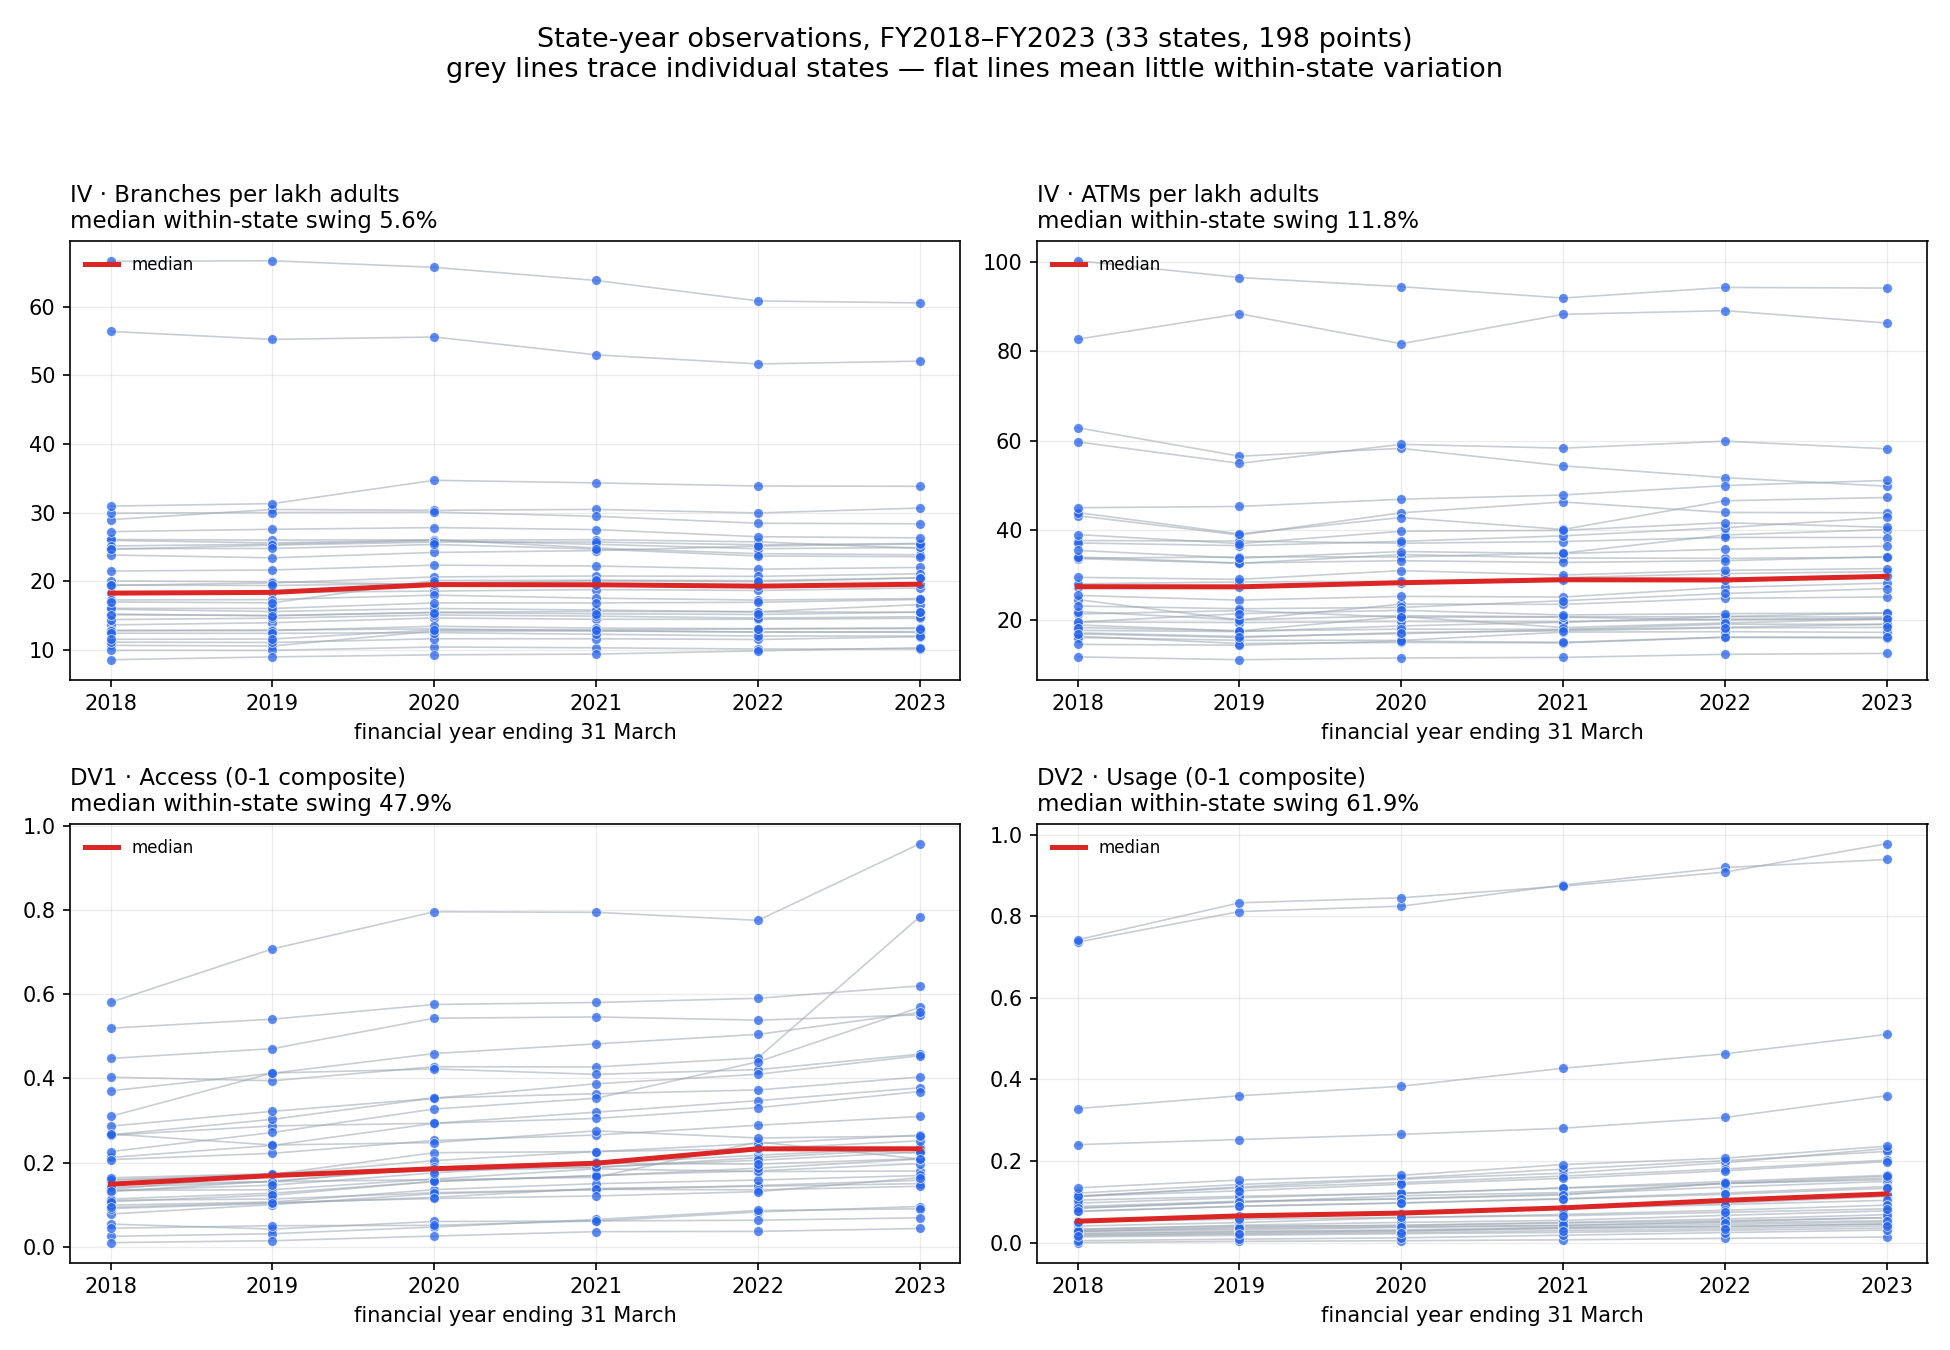
\includegraphics[width=\textwidth]{fig1_variables_over_time.png}
\caption{The identification problem. Each grey line traces one state across \panelA{}; the red line
is the cross-state median. \textbf{Top row, the regressors:} state lines run flat, with median
within-state swings of 5.6 per cent (branches) and 11.8 per cent (ATMs). \textbf{Bottom row, the
outcomes:} the same states climb steadily, swinging 47.9 and 61.9 per cent. Fixed effects use only
the vertical movement of individual lines, and there is very little of it in the top row.}
\label{fig:overtime}
\end{figure}

\subsection{Why the physical variation is so thin}

Three mechanisms compound, diagnosed before any coefficient was examined. \textbf{Infrastructure
stocks are slow-moving:} raw branch counts swing a median of only 10.7 per cent within a state
across six years --- 3.6 per cent in Chandigarh, 3.7 in Punjab. \textbf{The denominator cancels
much of what remains:} adult population grows a median 10.2 per cent within states over the window,
in the \emph{same direction} as branches, so branches per lakh adults swing only 5.6 per cent;
because the adult series is interpolated (Section~\ref{sec:data-defects}) it is almost perfectly
smooth and contributes no independent variation, merely deflating a trend. \textbf{The outcomes
move five to ten times more than the regressors:} credit accounts have a 30.0 per cent within share
against 7.0 for branches. Wide standard errors are guaranteed by construction, whether or not an
effect exists.

The problem is confined to the regressors --- the outcomes and the control have ample within-state
variation. The panel is not too short in general; it is too short \emph{for physical
infrastructure}. Lengthening the window helps but does not cure: the within share for branches
rises from 7.0 per cent over six years to 13.4 over ten, 20.1 over twelve, and 23.2 over thirteen,
still short of the PASS line. ATMs cannot follow at all, since the state-wise release begins in
2018. This is what motivates Track~2, and ultimately what motivates Track~3.

\section{Tracks 1 and 2: physical infrastructure}
\label{sec:h1-physical}

\begin{table}[H]
\centering
\caption{Two-way fixed-effects estimates, physical infrastructure. State and year effects
throughout; standard errors clustered by state. Track~2 drops ATMs, which cannot be extended
before 2018.}
\label{tab:physical}
\footnotesize
\begin{threeparttable}
\begin{tabular}{@{}llrrrrrr@{}}
\toprule
& & \multicolumn{3}{c}{Track 1 --- \panelA{}, $N=198$}
  & \multicolumn{3}{c}{Track 2 --- \panelB{}, $N=384$} \\
\cmidrule(lr){3-5}\cmidrule(lr){6-8}
Equation & Regressor & Coef. & SE & $p$ & Coef. & SE & $p$ \\
\midrule
\multirow{2}{*}{(1) \Access{}}
 & Branches & $-0.00897$ & 0.00699 & 0.201 & $-0.00483$ & 0.00645 & 0.455 \\
 & ATMs     & $-0.00164$ & 0.00377 & 0.664 & \multicolumn{3}{c}{---} \\
\addlinespace
\multirow{2}{*}{(2) \Usage{}}
 & Branches & $\mathbf{-0.01264}$ & 0.00363 & $\mathbf{0.001}$
            & $\mathbf{-0.01032}$ & 0.00570 & $\mathbf{0.071}$ \\
 & ATMs     & $-0.00109$ & 0.00263 & 0.678 & \multicolumn{3}{c}{---} \\
\addlinespace
\multirow{2}{*}{(3) \AUG{}}
 & Branches & $+0.00367$ & 0.00558 & 0.512 & $+0.00549$ & 0.00385 & 0.155 \\
 & ATMs     & $-0.00055$ & 0.00159 & 0.731 & \multicolumn{3}{c}{---} \\
\midrule
\multicolumn{8}{@{}l}{Within-$R^2$ --- Track 1: 0.069, 0.042, 0.111.
 Track 2: $-0.172$, $-0.478$, 0.215.} \\
\multicolumn{8}{@{}l}{Joint test (Track 1, Branch $=$ ATM $=$ 0): \Access{} $p = 0.374$;
 \Usage{} $p = 0.0005$; \AUG{} $p = 0.710$.} \\
\bottomrule
\end{tabular}
\begin{tablenotes}\scriptsize
\item The identity $\theta = \beta - \delta$ holds exactly throughout: for Track~1 branches,
$-0.00897 - (-0.01264) = +0.00367$. Track~2's negative within-$R^2$ values are reported rather than
suppressed; with two-way fixed effects the measure can go negative, and here it indicates the
regressors add nothing over the fixed effects alone.
\end{tablenotes}
\end{threeparttable}
\end{table}

\noindent
Read before interpretation: \textbf{nothing is significant in the \Access{} equation} on either
track, and every coefficient there is \emph{negative}. \textbf{Exactly one coefficient is
significant --- branches on \Usage{}, and it is negative.} \textbf{\AUG{} is not significant} for
any regressor on either track, so the formal test of the hypothesis returns nothing.
\textbf{ATMs are insignificant everywhere.} Explanatory power is very low throughout, exactly as
the gate forecast.

\begin{figure}[H]
\centering
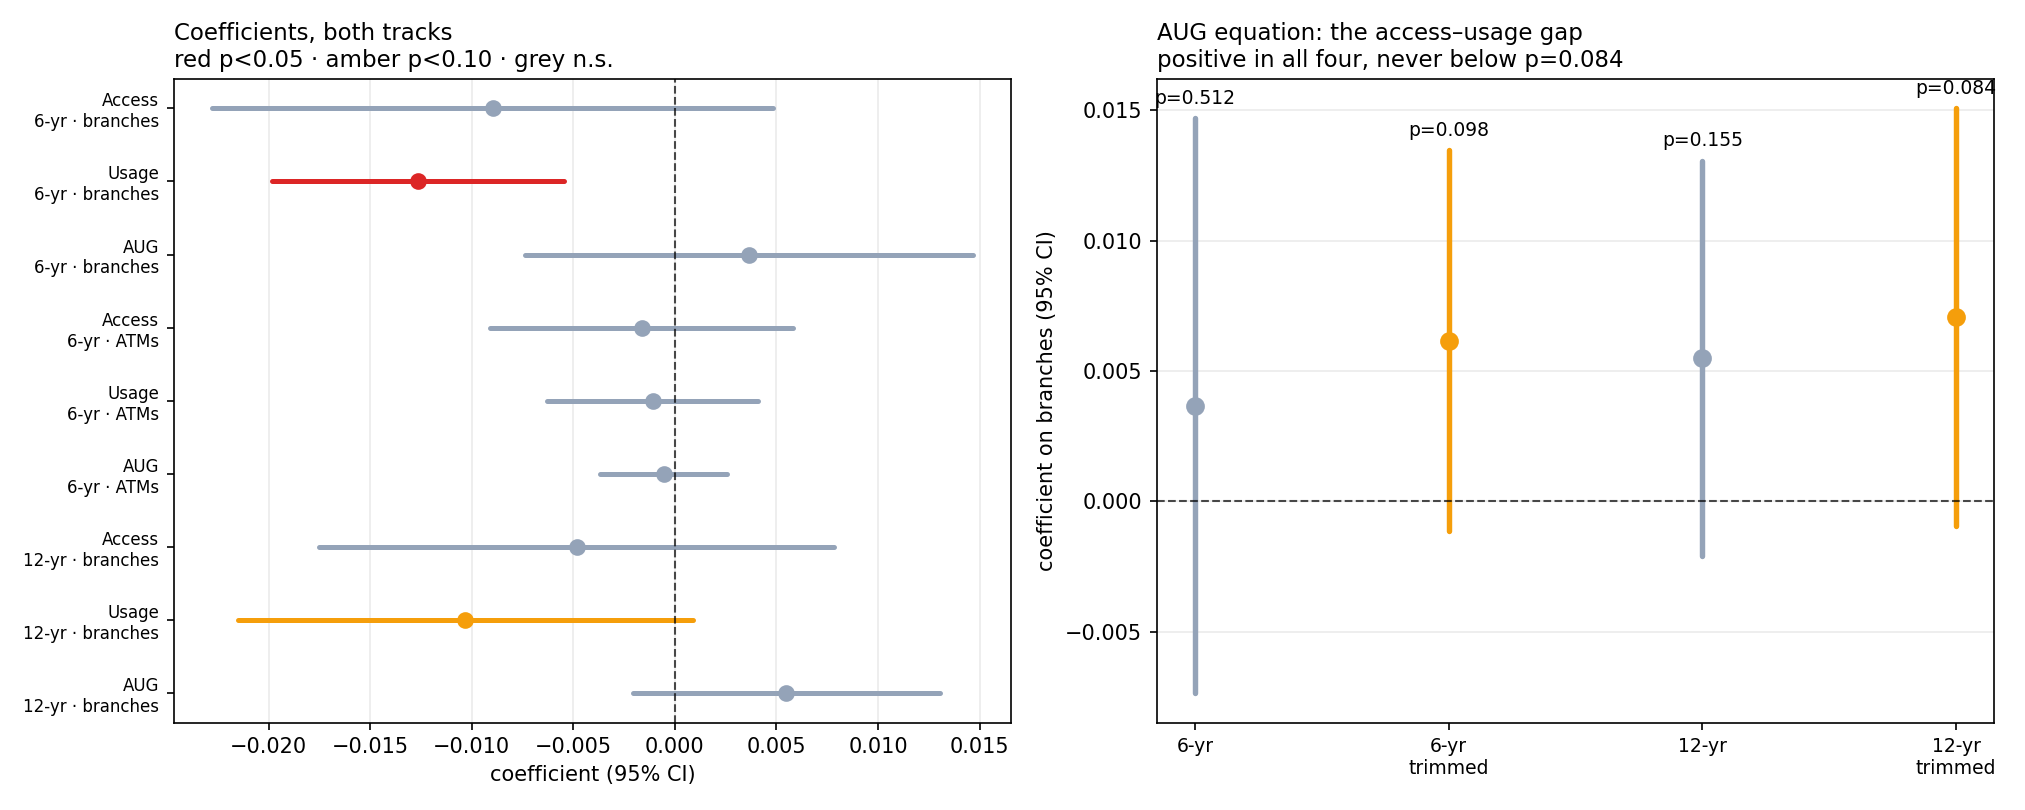
\includegraphics[width=\textwidth]{fig2_coefficients.png}
\caption{\textbf{Left:} every physical-infrastructure coefficient across both tracks, with 95 per
cent confidence intervals. Exactly one --- branches on \Usage{} in Track~1 --- is significant at
the 5 per cent level, and it is negative. \textbf{Right:} the coefficient on branches in the
\AUG{} equation across all four physical specifications. It is positive in every one, in the
direction the hypothesis predicts, but never attains conventional significance: $p$ runs $0.512$,
$0.098$, $0.155$, $0.084$. Reporting this as a finding would mean loosening the pre-committed rule
after seeing the coefficients, so it is recorded as a suggestive pattern only.}
\label{fig:coefs}
\end{figure}

\subsection{Random effects is not an escape}

Random effects would use both within- and between-state variation, and so appears to solve the
problem. The Hausman test asks whether doing so is consistent, under the null that state effects
are uncorrelated with the regressors \citep{hausman1978}. On Track~1 the null is rejected
decisively in all three equations ($\chi^2 = 108.3$, $73.2$ and $12.4$; $p < 0.0001$, $<0.0001$ and
$0.006$). State effects \emph{are} correlated with branches and ATMs --- the ``wealthier states
attract more infrastructure'' channel, confirmed rather than assumed. On Track~2 the evidence is
weaker: \Access{} now favours random effects ($p = 0.164$), while \Usage{} and \AUG{} still favour
fixed effects.

\begin{keybox}{The bind}
The Hausman test says fixed effects are \textbf{required}. The variance decomposition says fixed
effects have almost \textbf{nothing to work with}. Dropping the state fixed effects to recover
precision is not available --- the data itself rejects that specification. The design cannot be
rescued by changing estimator.
\end{keybox}

\subsection{Two observations decide the ATM result}
\label{sec:h1-robustness}

All equations were re-estimated dropping the two known-defective observations identified in
Section~\ref{sec:data-defects} --- Delhi 2023 and Chandigarh 2023, two cells out of 198.

\begin{table}[H]
\centering
\caption{Track~1 estimates against estimates excluding Delhi 2023 and Chandigarh 2023}
\label{tab:robustness}
\footnotesize
\begin{tabular}{@{}llrrrrl@{}}
\toprule
& & \multicolumn{2}{c}{Main ($N=198$)} & \multicolumn{2}{c}{Trimmed ($N=196$)} & \\
\cmidrule(lr){3-4}\cmidrule(lr){5-6}
Equation & Regressor & Coef. & $p$ & Coef. & $p$ & Change \\
\midrule
\Access{} & Branches & $-0.00897$ & 0.201 & $-0.00570$ & 0.078 & \\
\Access{} & \textbf{ATMs} & $\mathbf{-0.00164}$ & 0.664 & $\mathbf{+0.00331}$ & $\mathbf{0.004}$
  & \textbf{sign flip; becomes significant} \\
\addlinespace
\Usage{}  & Branches & $-0.01264$ & \textbf{0.001} & $-0.01185$ & \textbf{0.000} & stable \\
\Usage{}  & \textbf{ATMs} & $-0.00109$ & 0.678 & $+0.00011$ & 0.957 & \textbf{sign flip} \\
\addlinespace
\AUG{}    & Branches & $+0.00367$ & 0.512 & $+0.00615$ & 0.098 & \\
\AUG{}    & \textbf{ATMs} & $-0.00055$ & 0.731 & $+0.00319$ & 0.148 & \textbf{sign flip} \\
\bottomrule
\end{tabular}
\end{table}

\begin{keybox}{Two observations out of 198 reverse the sign of every ATM coefficient}
They also move the estimated effect of ATMs on \Access{} from null ($p = 0.664$) to significant and
positive ($p = 0.004$). A result that depends on two state-years is not a result: \textbf{nothing
about ATMs can be concluded in either direction.}
\end{keybox}

\noindent
This is what the gate predicted. When a regressor carries only 7 to 9 per cent within-state
variation, individual observations acquire enormous leverage. The two dropped cells are moreover
\emph{known defects in RBI's published source}, not outliers chosen for being inconvenient --- so
the headline ATM result had been riding on data already established as wrong. On Track~2, with the
window doubled and within-state variation at 15.3 per cent, the same trim produces \textbf{no sign
flips anywhere}: the fragility disappears with more data, though the verdict does not change.

\section{Track 3: substituting the infrastructure that moved}
\label{sec:h1-digital}

\subsection{Why}

Over \panelA{}, physical banking infrastructure in India was flat while retail payments moved onto
phones. If financial infrastructure was doing anything over this window, it was not doing it
through branches. Figure~\ref{fig:premise} states that premise in numbers.

\begin{figure}[H]
\centering
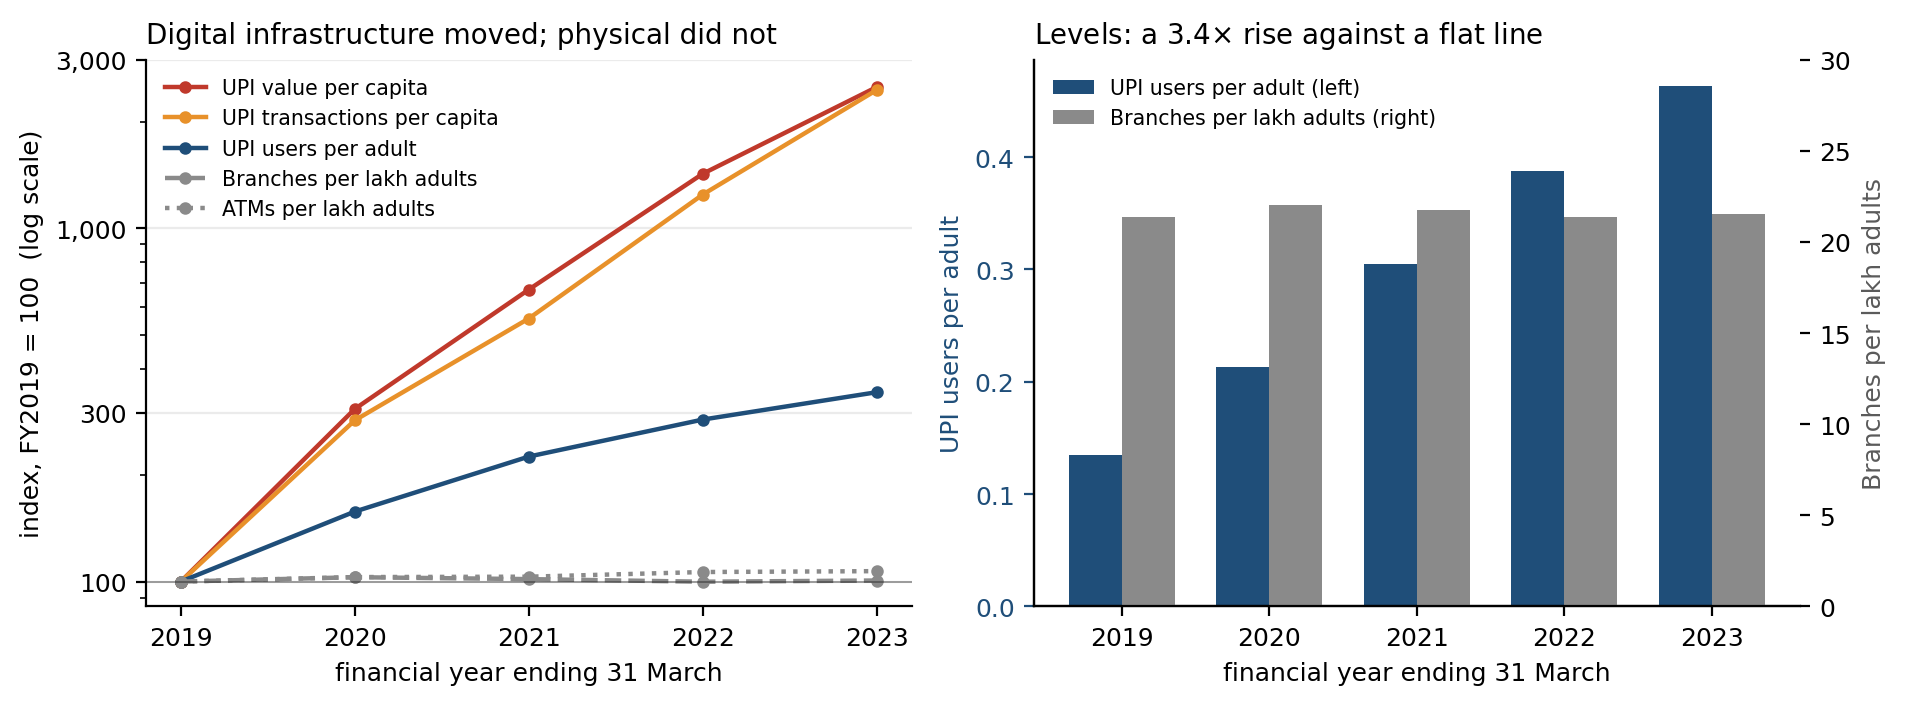
\includegraphics[width=\textwidth]{fig4_digital_vs_physical.png}
\caption{\textbf{Left:} unweighted state means indexed to FY2019, on a log scale. UPI value and
transactions per capita rise roughly twenty-five-fold in five years; branches and ATMs per lakh
adults are flat. \textbf{Right:} the same in levels --- UPI users per adult rise from 0.135 to
0.464 while branches per lakh adults sit between 21.4 and 22.0 throughout.}
\label{fig:premise}
\end{figure}

\begin{figure}[H]
\centering
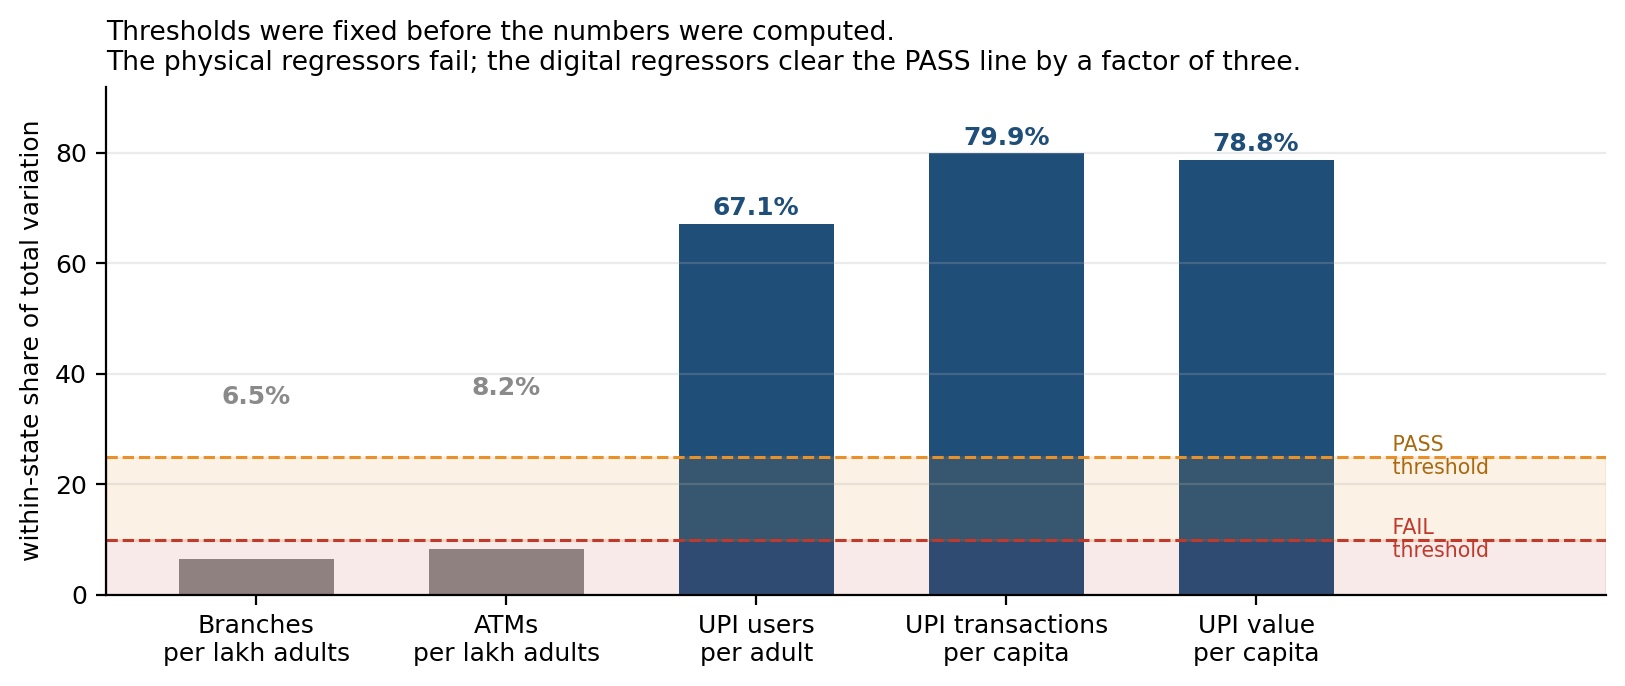
\includegraphics[width=0.92\textwidth]{fig5_within_variation.png}
\caption{Within-state share of total variation, against thresholds fixed before the numbers were
computed. The reason Tracks~1 and~2 could not test the hypothesis does not apply to Track~3.}
\label{fig:variation}
\end{figure}

\noindent
The consequence for estimation is immediate. Within-state variation in UPI users per adult is
\textbf{67.1 per cent}, against 6.5 for branches and 8.2 for ATMs on the same sample. Explanatory
power rises correspondingly: within-$R^2$ goes from 0.069 to \textbf{0.609} for \Access{} and from
0.042 to \textbf{0.863} for \Usage{}. Fixed effects plus branches and ATMs explained essentially
nothing; one digital variable explains most of it.

\subsection{The test that mattered}
\label{sec:h1-decomp}

One objection has to be dealt with before any digital coefficient can be read. PhonePe registration
requires a KYC-linked bank account, so UPI adoption and \emph{deposit-account counts} are entangled
by accounting rather than by economics --- the same trap that dropping PMJDY was meant to avoid,
and deposit accounts are half of the \Access{} construct. Credit accounts are not entangled the
same way: a bank loan account is neither required for nor created by PhonePe registration.

The outcome was therefore decomposed into its four underlying indicators, with the reading fixed
before the regressions were run (D17): if UPI $\to$ credit accounts is large and significant, the
\Access{} result is not merely definitional; if credit is null while deposits are large, the
\Access{} coefficient \emph{is} the accounting relationship and \Access{} must be reported
credit-only thereafter; if both are large, only the credit result gets a substantive reading.

\begin{figure}[H]
\centering
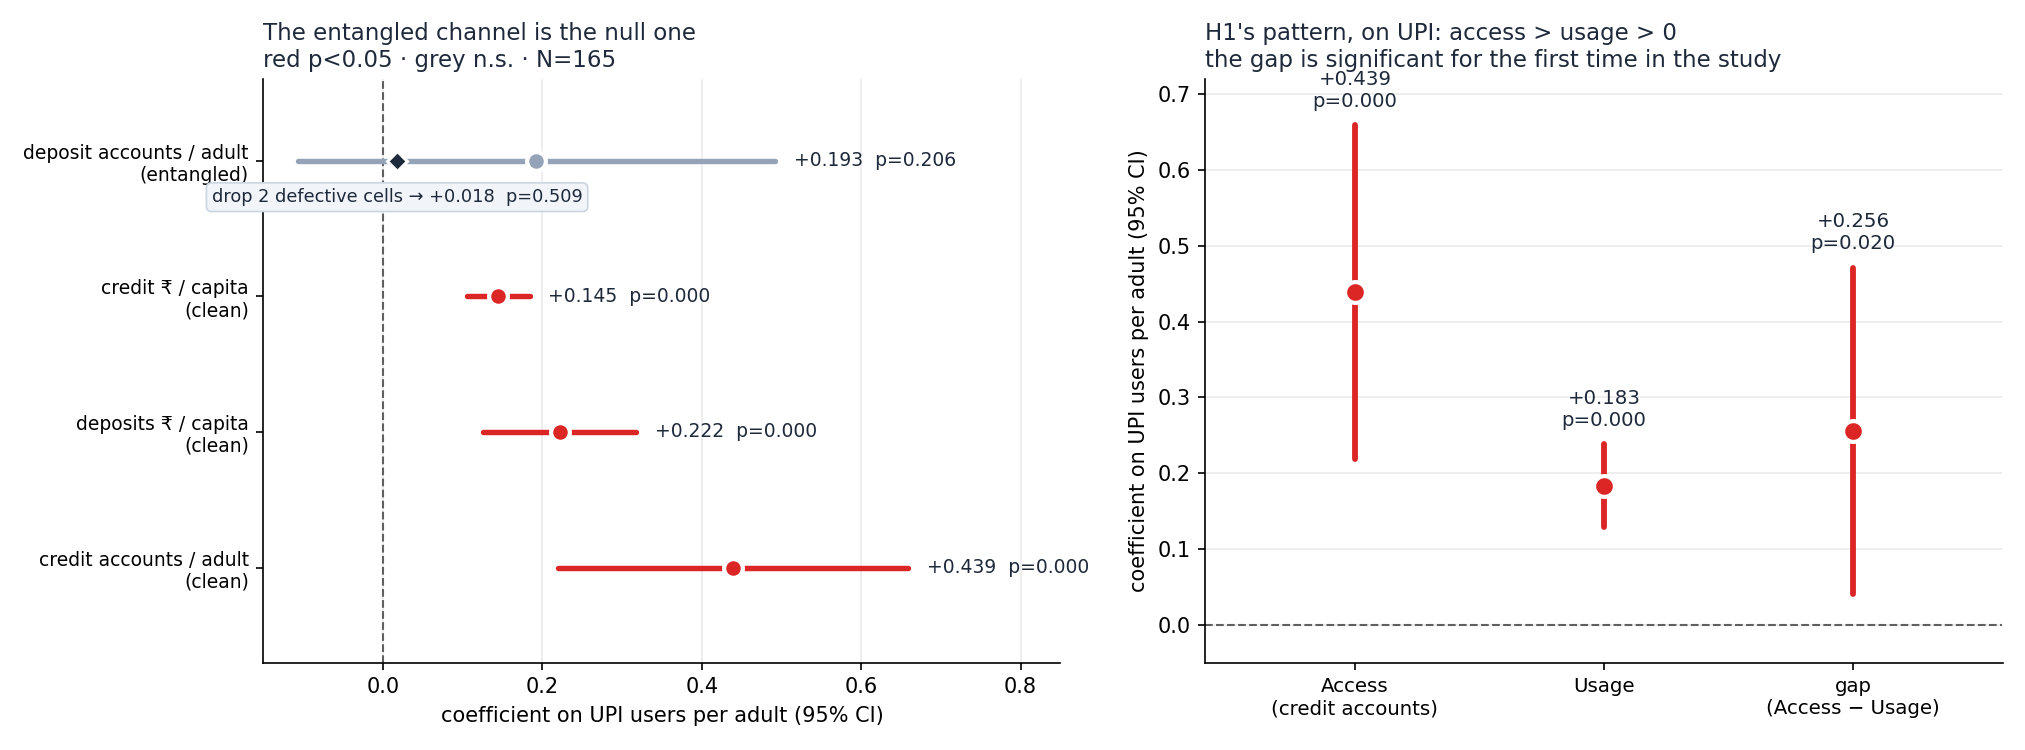
\includegraphics[width=\textwidth]{fig3_digital.png}
\caption{\textbf{Left:} the coefficient on UPI users per adult for each of the four outcome
components. The entangled channel is the null one, and collapses further when the two defective
cells are dropped. \textbf{Right:} the hypothesis pattern on the credit-only specification.}
\label{fig:digital}
\end{figure}

\begin{table}[H]
\centering
\caption{Component decomposition: coefficient on UPI users per adult, $N=165$, and the same
estimate excluding Delhi 2023 and Chandigarh 2023}
\label{tab:components}
\footnotesize
\begin{tabular}{@{}llrrrr@{}}
\toprule
Component & Status & Coef. & $p$ & Coef. (trimmed) & $p$ \\
\midrule
Deposit accounts per adult & \textbf{entangled} & $+0.193$ & 0.206 & $+0.018$ & 0.509 \\
Credit accounts per adult  & clean & $\mathbf{+0.439}$ & $\mathbf{0.0001}$ & $+0.445$ & 0.0003 \\
Deposits \rs per capita    & clean & $+0.222$ & $<0.001$ & --- & --- \\
Credit \rs per capita      & clean & $+0.145$ & $<0.001$ & --- & --- \\
\addlinespace
\Access{} (composite)      & mixed & $+0.316$ & 0.0004 & $+0.231$ & 0.0005 \\
\bottomrule
\end{tabular}
\end{table}

\begin{keybox}{The concern was not merely unfounded --- it pointed the wrong way}
The \textbf{entangled} channel is the null one: UPI $\to$ deposit accounts is $+0.193$
($p = 0.206$), collapsing to $+0.018$ ($p = 0.509$) when the two known-defective cells are dropped,
with the standard error falling from 0.151 to 0.027. The \textbf{clean} channel carries everything:
UPI $\to$ credit accounts is $+0.439$ ($p = 0.0001$) and is completely unmoved by the same trim.

\medskip
The entangled component was \emph{diluting} a real credit effect, not manufacturing one. The
composite \Access{} number averages a genuine effect with a defect-driven artefact, so
\textbf{\Access{} is reported credit-only from here}.
\end{keybox}

\subsection{The hypothesis pattern, on the credit-only specification}

\begin{table}[H]
\centering
\caption{Track~3, credit-only \Access{}. Two-way fixed effects, $N = 165$, standard errors
clustered by state}
\label{tab:digital}
\small
\begin{tabular}{@{}lrrr@{}}
\toprule
Regressor & \Access{} (credit accounts) & \Usage{} & Gap (\AUG{}) \\
\midrule
\textbf{UPI users per adult} & $\mathbf{+0.439}$ ($p<0.001$) & $\mathbf{+0.183}$ ($p<0.001$)
  & $\mathbf{+0.256}$ ($\mathbf{p=0.020}$) \\
Branches per lakh adults & $+0.0091$ ($p=0.085$) & $-0.0062$ ($p=0.020$) & $+0.0153$ ($p=0.018$) \\
ATMs per lakh adults & $-0.0007$ ($p=0.773$) & $-0.0002$ ($p=0.868$) & $-0.0005$ ($p=0.884$) \\
\bottomrule
\end{tabular}
\end{table}

\noindent
Four things follow. \textbf{For UPI, $\beta_{\text{access}} > \beta_{\text{usage}} > 0$ and the gap
is significant at 5 per cent} --- the pattern the hypothesis predicts, and the first time in this
study that the access--usage gap is distinguishable from zero. \textbf{Branches turn positive on
access for the first time}, once \Access{} is credit-only and digital adoption is controlled for,
though only at $p = 0.085$. \textbf{ATMs are null on everything}, and the ATM coefficient that
looked significant under trimming in Track~1 is revealed as a composite-outcome artefact.
\textbf{Physical infrastructure still fails the pre-committed rule}, and that verdict never
changed.

\subsection{Robustness}

The headline coefficient was refit 33 times, dropping each state in turn.

\begin{figure}[H]
\centering
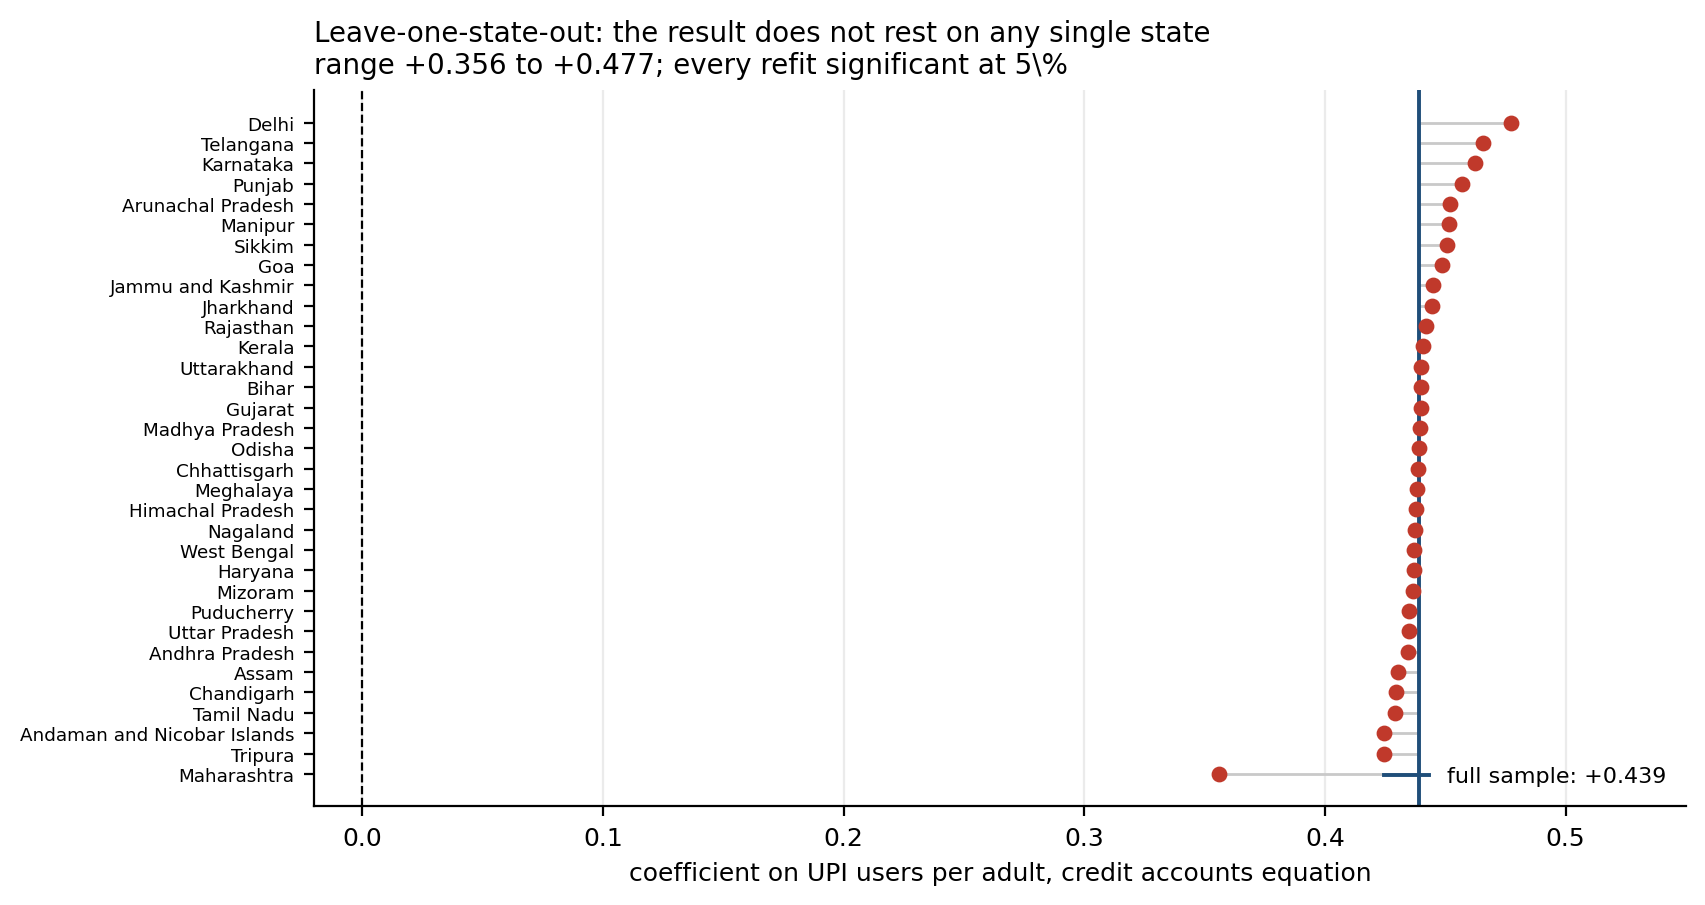
\includegraphics[width=0.95\textwidth]{fig6_leave_one_out.png}
\caption{Leave-one-state-out estimates of the coefficient on UPI users per adult in the credit
accounts equation. The estimate stays between $+0.356$ and $+0.477$, and no refit loses
significance at the 5 per cent level. Maharashtra is the most influential single state, and the
result is \emph{stronger} without it.}
\label{fig:loo}
\end{figure}

\noindent
The contrast with Track~1 is the point: there, two cells out of 198 flipped every ATM sign; here,
removing an entire state moves the coefficient by at most 19 per cent and never changes the
conclusion. The result is also unmoved by the D7 data defects, which affect savings accounts and
therefore cannot touch a credit-only outcome.

\subsection{A mechanism that fits}

Digital payment history feeding credit underwriting --- cash-flow-based lending, and the account
aggregator framework --- is a documented development in India over exactly this window, and the
wider literature finds digital payment adoption spreading through network effects rather than
infrastructure stock \citep{crouzet2023,dsilva2019}. It predicts precisely what is observed: UPI
moving loan accounts while leaving deposit accounts alone. That the data is consistent with a
mechanism is suggestive of it, not proof.

\section{Verdict}
\label{sec:h1-verdict}

\subsection{Against the pre-committed rule}

The rule requires $\beta_{\text{access}} > \beta_{\text{usage}} > 0$ for branches \emph{and} ATMs.
For branches on Track~1, the ordering holds ($-0.00897 > -0.01264$) but both coefficients are
negative, so the positivity condition fails; the difference is insignificant ($p = 0.512$). For
ATMs the ordering does not hold, nothing is significant, and every sign reverses on a two-cell
trim. Track~2 reproduces the branch result with twice the power and none of the fragility.

\begin{keybox}{Verdict on the pre-committed hypothesis}
\textbf{Hypothesis 1 is not supported for physical infrastructure.} This is not partial support:
the positivity condition fails for branches, and the ordering condition fails for ATMs. The same
conclusion is reached on all three tracks, and it never changed.
\end{keybox}

\noindent
Mapping onto the outcomes tabulated in advance, the row that applies is \emph{both effects
$\approx 0$ --- check within-state variation before concluding anything}. The diagnostic was run
first, as instructed, and returned 7.0 and 8.7 per cent. The correct conclusion is therefore
\textbf{not} that infrastructure fails to raise financial inclusion, but that \textbf{Tracks~1
and~2 cannot test the question}: the regressors barely move, the estimator the Hausman test
requires discards the variation that does exist, and the estimates are unstable to two
observations. The null is uninformative, exactly as fixed in advance that it would be.

\subsection{What the digital result is, and what it is not}
\label{sec:h1-exploratory}

\begin{keybox}{The digital result is exploratory by construction}
The pre-committed rule named \textbf{branches and ATMs}, and it failed. \textbf{UPI was added after
seeing that null.} The digital finding therefore cannot be reported as a hypothesis that was tested
and passed --- it is a hypothesis \textbf{generated} by this data, for a future design to test.
Stating it any other way is exactly the retro-fitting that pre-committing was meant to prevent.
\end{keybox}

\noindent
This is the first thing a careful reader will test, so it is stated here rather than buried. What
can be said is bounded but not trivial: on a measure of financial infrastructure that genuinely
moved within states, the access--usage gap widens significantly, the effect runs entirely through
the channel that is not definitionally entangled with the regressor, and the result survives the
removal of any single state. The identification problem that defeated Tracks~1 and~2 is solved. The
causal problem is not --- fixed effects remove fixed state differences and the common national
trend, but not state-specific time-varying confounders, and smartphone penetration, fintech entry
and youth share all rose alongside both UPI adoption and credit accounts over these five years.

\subsection{The persistent puzzle}

One physical coefficient is significant and robust across specifications: \textbf{branches on
\Usage{}, negative} ($p = 0.001$ on Track~1, $0.071$ on Track~2, $0.020$ on Track~3). Within a
state, years with more branches per lakh adults show lower \Usage{}. It is the opposite sign to
anything the hypothesis anticipated, and it is treated as a puzzle rather than a result: the
variation problem applies to it as much as to the nulls, \Usage{} is severely compressed by the
pooled normalisation, and a negative within-state relationship is at least as consistent with
branches being \emph{placed} where deposit growth is weak as with branches causing it. Nothing here
identifies direction.

\section{Limitations}
\label{sec:h1-limitations}

Ordered by how much damage each does to the conclusions.

\paragraph{1. Identification --- the binding limitation.} On the physical tracks the regressors
barely move: 7.0 and 8.7 per cent within-state variation, below the FAIL threshold fixed before
looking. The null on branches and ATMs \textbf{cannot be distinguished from ``not enough variation
to detect anything''}, and any such null must be reported with these numbers attached. On the
digital track variation is ample and that objection does not apply --- but fixed effects do not
remove state-specific time-varying confounders, so the digital result is a within-state correlation
between two co-trending series and \textbf{no causal claim is available}. Reverse causality is live
rather than hypothetical: the Hausman test rejecting random effects is direct evidence that state
effects are correlated with the regressors.

\paragraph{2. The digital result is exploratory by construction.} UPI was added after seeing the
physical null (Section~\ref{sec:h1-exploratory}).

\paragraph{3. Known data defects.} The deposit-account breaks in RBI's source (Delhi 2023,
Chandigarh 2023 inside the window) were enough to move the deposit-account coefficient from
$+0.193$ to $+0.018$. Adult population is interpolated rather than published for 243 of 266
state-years, and being near-linear it \emph{suppresses} within-state variation in the per-adult
regressors, making the first limitation worse than it looks. Two units are dropped for want of
income data, and boundary changes forced merges, so nothing state-specific can be said about
either half of a merged unit.

\paragraph{4. Measurement.} \textbf{Attribution differs three ways:} bank deposits and credit are
recorded at branch location, loan accounts by place of sanction, and PhonePe by the user's
registered state --- three different definitions of ``where'', merged into one panel. The first
inflates Maharashtra and Delhi, where lending is booked. \textbf{PhonePe is one firm}, roughly
45--50 per cent of UPI, with market share varying by state, so cross-state levels are noisier than
within-state growth; NPCI's total UPI series would fix this. \textbf{\Usage{} is severely
right-skewed after normalisation} --- 85 per cent of observations below 0.20 --- so
$\beta_{\text{access}}$ and $\beta_{\text{usage}}$ were never on fully equivalent scales, a direct
threat to the comparison itself, left unfixed deliberately in order to test the specification as
written. And the study is \textbf{state-level, not person-level}: nothing here can show that
\emph{individuals} hold unused accounts, which is the mechanism the hypothesis describes.

\paragraph{5. Scope.} The physical panel stops at FY2023, FY2024 having been traded away for a
consistent bank universe; the digital panel is five years, since PhonePe data begin in 2018; ATMs
cannot extend before 2018; and dropping PMJDY, though necessary, left the physical measure with
nothing digital in it until PhonePe was added.

\begin{keybox}{What survives all of this}
The \textbf{physical null}, reported as uninformative rather than as evidence of no effect.
\textbf{Branches $\to$ \Usage{} negative} ($p \leq 0.020$ across three specifications and two
samples), robust but with no causal reading available. \textbf{UPI $\to$ credit accounts positive}
($+0.439$), robust to dropping any single state and to the known data defects --- but
correlational. And \textbf{UPI $\to$ deposit accounts $\approx 0$}, which is the asymmetry the whole
digital finding rests on.
\end{keybox}

\input{chapters/04_hypothesis2}
%=====================================================================
%  CHAPTER STUB --- HYPOTHESIS 3
%  Mirrors Chapter~\ref{ch:h1} section for section, so the three
%  hypotheses read comparably. Replace the title, then fill each
%  section in order. Every \label{} used by cross-references already
%  exists, so the document compiles while this chapter is empty.
%=====================================================================
\chapter{Hypothesis 3: [Title to be supplied]}
\label{ch:h3}

\section{Hypothesis and pre-commitment}
\label{sec:h3-hypothesis}

\begin{keybox}{Hypothesis 3}
\textit{[Statement to be supplied.]}

\medskip
\emph{Rationale.} \textit{[The mechanism, not the expectation.]}
\quad \emph{Expected:} \textit{[The sign pattern that would constitute support.]}
\end{keybox}

\stub{Fix the decision rule \textbf{before} estimating, as D10 does in
Section~\ref{sec:h1-hypothesis}: what counts as full support, what counts as partial support, and
that it will not be revised after the coefficients are seen. Log it in Appendix~\ref{app:decisions}
with its own D-number.}

\section{Variables and specification}
\label{sec:h3-variables}
\label{sec:h3-spec}

\stub{Define the independent, dependent and control variables with units and denominators, then
state the estimating equation(s), fixed-effects structure, and clustering. Chapter~\ref{ch:data}
documents the shared panel --- reference it rather than repeating it, and add any series not in
Table~\ref{tab:sources}.}

\section{Descriptives and diagnostics}
\label{sec:h3-descriptives}
\label{sec:h3-diagnostics}

\stub{Means, standard deviations and ranges, flagging anything bearing on the specification ---
skew, compression, extreme values --- \textbf{before} presenting estimates. Then run the
within-state variance decomposition first, with thresholds fixed before the numbers are computed
(Section~\ref{sec:h1-gate}), and report the verdict whether or not it is favourable.}

\section{Results and robustness}
\label{sec:h3-results}
\label{sec:h3-robustness}

\stub{Main estimates, reported before they are interpreted. Then re-estimate excluding the
known-defective cells of Section~\ref{sec:data-defects}, plus any perturbation specific to this
hypothesis, reporting sign and significance changes explicitly.}

\section{Verdict, implications and limitations}
\label{sec:h3-verdict}
\label{sec:h3-implications}
\label{sec:h3-limitations}

\stub{Apply the pre-committed rule as written; state whether the hypothesis is supported,
partially supported or not supported, and what the result does \textbf{not} license concluding.
Then substantive, policy and methodological implications, carrying the cross-cutting ones to
Chapter~\ref{ch:conclusion}; then limitations, referencing rather than restating the shared data
limitations of Section~\ref{sec:data-defects}.}

\chapter{Discussion and Conclusion}
\label{ch:conclusion}

\section{Synthesis}
\label{sec:synth}

\paragraph{Hypothesis 1.} The claim was that financial infrastructure raises access more than usage
--- that expansion is formal rather than functional. Measured physically, as branches and ATMs, it
is \textbf{not supported}, and the more consequential result is why. Only 7.0 per cent of the
variation in branches per lakh adults, and 8.7 per cent of that in ATMs, occurs within states;
roughly 93 per cent is cross-sectional, which is precisely what fixed effects discard. The Hausman
test then rejects random effects, closing off the specification that would have used that
variation, and two defective observations out of 198 prove enough to reverse the sign of every ATM
coefficient. Doubling the window to twelve years doubles the usable variation and removes the
fragility, but leaves the verdict unchanged.

Measured digitally, the picture reverses. UPI adoption varies 67.1 per cent within states over the
same window, explanatory power rises roughly ninefold, and the predicted pattern appears:
$\Access{} +0.439$, $\Usage{} +0.183$, gap $+0.256$ at $p = 0.020$. The effect runs entirely
through credit accounts and not at all through deposit accounts --- the opposite of what an
accounting artefact would produce, since deposit accounts are the component entangled with UPI
registration by construction. The asymmetry is the finding. But UPI entered the design after the
physical null was seen, so this is a hypothesis generated by the data rather than one tested and
passed.

\stub{Summarise the verdicts on Hypotheses 2 and 3 here in the same form --- what was claimed, what
was found, what the result does not license --- then add a short paragraph on whether the three
point in a common direction. If they share the panel of Chapter~\ref{ch:data}, note explicitly
whether the within-state variation problem of Section~\ref{sec:h1-gate} affects them too: it is a
property of the data, not of Hypothesis~1.}

\section{Implications for policy}
\label{sec:policy}

\paragraph{Measure usage, not ownership.} Account ownership is near saturation, and the marginal
account opened now is very likely to be dormant: roughly 35 per cent of Indian adults with an
account hold an inactive one \citep{findex2021}, and about 26 per cent of PMJDY accounts are
reported inoperative \citep{pmjdy2025}. The RBI's Financial Inclusion Index already weights usage
(45 per cent) above access (35 per cent) \citep{rbi_fiindex2025}, and the evidence here supports
that ordering. Targets expressed in accounts opened measure the dimension that is no longer
binding.

\paragraph{The binding infrastructure has changed, and measurement should follow.} Branches per
lakh adults move a median of 5.6 per cent within a state over six years; UPI adoption moved by
orders of magnitude over the same period. Whatever the long-run effect of physical premises, they
are not the margin on which annual variation in financial inclusion was determined over
FY2019--FY2023. A framework that monitors branch and ATM density while treating digital payment
adoption as background is measuring the stationary part of the system.

\paragraph{If the credit channel is real, it is a policy object.} The digital result is
correlational, but the association it identifies --- digital payment adoption moving \emph{loan}
accounts while leaving deposit accounts untouched --- is consistent with payment history entering
credit underwriting, which is a deliberate feature of Indian financial architecture over this
period. That makes it a testable and governable channel rather than an incidental one, and it
sharpens what an evaluation should look for.

\paragraph{Data quality is itself a policy variable.} A discontinuity in one column of one RBI
return, affecting three states, was enough to reverse the sign of every ATM coefficient in Track~1
and to inflate a null deposit-account coefficient tenfold in Track~3. Series used for programme
evaluation warrant the revision and documentation discipline applied to headline aggregates.

\section{Implications for method}
\label{sec:method-implications}

\paragraph{Diagnose the identifying variation before estimating.} The variance decomposition was
specified as a gate, with thresholds fixed before the numbers were computed, and it correctly
forecast the instability the robustness checks later demonstrated. Had coefficients been examined
first, the null on \Access{} would have read as a substantive finding about infrastructure, and the
significant ATM coefficient under trimming as a discovery. Both readings would have been wrong, and
neither obviously so. The same statistic then did positive work: it is what identified digital
adoption as a regressor capable of answering the question, rather than merely another variable to
try. A wide confidence interval is ambiguous between ``there is no effect'' and ``there is no
variation from which to detect one'', and this distinction carries the whole report.

\paragraph{Decompose a composite outcome when any component is entangled with the regressor.} The
headline \Access{} coefficient on UPI would have been reportable as it stood. Splitting it revealed
that the entangled component was null and the clean component carried everything --- so the
composite was averaging a real effect with a defect-driven artefact, and the naive concern about
mechanical correlation pointed the wrong way. The rule for reading that decomposition was fixed
before it was run, which is what made the outcome interpretable either way.

\paragraph{Pre-registration is most valuable when results are ambiguous.} Had the estimates been
clean, the rule fixed in advance would have been redundant. They were not. It is also what forces
the honest statement of the digital result's status: the rule named branches and ATMs, so no
reading of the UPI finding can claim the hypothesis was tested and passed.

\paragraph{Slow-moving regressors and short panels are a recurring trap.} Infrastructure,
institutions and capital stocks all move slowly; two-way fixed effects is the default estimator;
and the Hausman test will typically forbid retreat to random effects in exactly the settings where
between-state variation is most correlated with the outcome. The reconsideration of
\citet{burgess2005} by \citet{buliskeria2022} makes the same point from the other direction. The
remedy applied here --- find the infrastructure that actually moved --- is more generally available
than it looks.

\section{Directions for further work}
\label{sec:further}

Three things would strengthen this, in order of value. \textbf{An identification strategy for UPI}
is the first and largest: the current digital result is a within-state correlation between two
co-trending series, and candidate instruments include state-level 4G rollout timing or the
staggered geography of Jio's 2016--17 entry. \textbf{Total UPI rather than one firm} would remove
the varying-market-share problem, since NPCI publishes state-level aggregates that would replace
the PhonePe proxy. \textbf{Extending the digital panel} would take it from five years to eight, the
PhonePe series running to FY2026 while the banking series stop at FY2023. Beyond these,
sub-state disaggregation would raise precision substantially, and three measurement problems are
tractable: replacing the interpolated adult denominator with Census-based age shares, estimating on
logs or ranks rather than pooled min--max levels to address the compression of \Usage{}, and
reconciling the three attribution rules currently merged into one panel.

\section{Conclusion}
\label{sec:conclusion}

This report asked whether the expansion of financial infrastructure in India has been formal rather
than functional --- whether it opens accounts faster than it puts them to use. The question is well
motivated: India has effectively solved account ownership while recording the highest rate of
account dormancy in the world.

Asked of \emph{physical} infrastructure, the question cannot be answered with these data.
Hypothesis~1 is not supported, but the null is uninformative: branches and ATMs do not move enough
within Indian states over six years, or even twelve, for a fixed-effects panel to detect their
effect, and the specification test that would license using cross-sectional variation instead
rejects that estimator decisively. Two observations out of 198 reverse the sign of every ATM
coefficient, which demonstrates the point rather than merely asserting it.

Substituting the infrastructure that actually moved changes the picture. UPI adoption varies
abundantly within states, and on that measure the predicted pattern appears: access rises more than
usage, and the gap between them is significantly different from zero for the first time in the
study. It does so entirely through credit accounts rather than deposit accounts --- an asymmetry
that is the reverse of what a mechanical artefact would generate, and one that fits a documented
channel, digital payment history feeding credit underwriting.

\begin{keybox}{The honest headline}
A state panel cannot identify the effect of \emph{physical} banking infrastructure on financial
inclusion, because branches and ATMs barely move within states. Substituting the infrastructure
that actually moved --- digital payments --- the picture reverses: UPI adoption predicts access
more strongly than usage, significantly so, and it does it entirely through credit accounts rather
than deposit accounts. \textbf{The identification problem is solved; the causal one is not.}
\end{keybox}

\noindent
Two boundaries must travel with that. The pre-committed hypothesis named branches and ATMs and it
failed; UPI was added afterwards, so the digital finding is a hypothesis this data \emph{generated}
and not one it tested. And fixed effects remove fixed state differences and the common national
trend, not state-specific time-varying confounders --- smartphone penetration, fintech entry and
youth share all rose alongside both UPI adoption and credit accounts.

What remains is a clear direction rather than a closed question. The variation this design needed
and did not have exists in abundance on the digital side; what it now lacks is exogeneity, not
power. That is a more tractable problem than the one it started with, and the discipline that made
this report's negative result legible --- fixing the decision rule and the diagnostic thresholds
before seeing the numbers --- is what should be carried into solving it.


%---------------------------------------------------------- BACK MATTER
\appendix
\chapter{Decision Log}
\label{app:decisions}

Every non-obvious choice taken during data preparation and estimation was recorded when it was
taken, with its rationale and consequences, in an append-only log, reproduced here in full. Its
purpose is auditability: each choice can be verified as made for a stated reason and --- for the
decisions constraining interpretation --- as made \emph{before} the results it constrains were
seen.

{\footnotesize
\begin{longtable}{@{}p{0.7cm}p{3.1cm}p{10.5cm}@{}}
\caption{Decision log, D1--D17}
\label{tab:decisionlog}\\
\toprule
\textbf{\#} & \textbf{Decision} & \textbf{Rationale and consequence} \\
\midrule
\endfirsthead
\multicolumn{3}{@{}l}{\small\itshape Table \ref{tab:decisionlog} continued from previous page}\\
\toprule
\textbf{\#} & \textbf{Decision} & \textbf{Rationale and consequence} \\
\midrule
\endhead
\midrule
\multicolumn{3}{r@{}}{\small\itshape continued on next page}\\
\endfoot
\bottomrule
\endlastfoot

D1 & Drop Lakshadweep and Dadra \& Nagar Haveli and Daman \& Diu &
No per-capita NSDP published for either in any year, so neither can carry the income control. 35 units become 33; both are very small. \\
\addlinespace

D2 & Merge J\&K with Ladakh, and DNH with Daman and Diu, in every year &
Boundaries changed mid-sample and fixed effects require each unit to mean the same thing throughout. Sources record the change in different years, so summing all components in all years is the only rule that works for every source at once. \\
\addlinespace

D3 & Drop PMJDY; infrastructure is branches and ATMs only &
Removes the only digital component, so the measure is \emph{physical banking infrastructure}. Later found load-bearing rather than cosmetic: PMJDY accounts are an account count, and retaining them would have put an account count on both sides of the regression. \\
\addlinespace

D4 & Keep Gujarat; leave its FY2023--24 income cell missing &
Not sourceable --- Gujarat is absent from every Handbook income table that year. Superseded by D8, which moves the cell outside the window. \\
\addlinespace

D5 & Year alignment: banking $Y$ $\equiv$ income $(Y{-}1)$--$Y$ $\equiv$ population 1 March $Y$ &
All stocks at 31 March; the easiest place to introduce a silent one-year offset. Implemented as a canonical column in D9. \\
\addlinespace

D6 & Disclose that adult population is interpolated &
Age structure is published only every five years; 243 of 266 state-years use an estimated 18+ share applied to published annual totals. \\
\addlinespace

D7 & Keep Delhi, Haryana and Chandigarh despite defective deposit-account values &
The savings-account column jumps discontinuously (Delhi 39m to 106m in 2023; Haryana 53m to 102m in 2024; Chandigarh spikes in 2023 and reverts). Extraction is correct --- the break is in RBI's source. Retain in the main specification, then re-run without them as a robustness check. \\
\addlinespace

D8 & Switch loan accounts to the RRB-inclusive file; panel becomes FY2018--FY2023 &
Fixes a bank-universe mismatch so every variable counts the same banks. The files could not be merged arithmetically --- they also differ on \emph{where} a loan is counted, and differencing gave impossible negative values for Maharashtra. Cost: FY2024. Benefit: removes the Gujarat gap, leaving 198 balanced rows. \\
\addlinespace

D9 & Add one canonical year column, \texttt{fy\_end}, to all eight files &
\texttt{fy\_end} is the calendar year of the 31 March a row refers to; merge, filter and take the year fixed effect on it. Only the income file needed converting; native labels retained so the original coding stays auditable. Not named plain \texttt{year}, because a bare \texttt{2018} is exactly the ambiguity that causes the bug. \\
\addlinespace

D10 & No composite index; branches and ATMs enter as two separate regressors. \textbf{Final} &
Raw correlation 0.904 is almost entirely cross-sectional; after demeaning it falls to 0.305, VIF 1.10. Removes two arbitrary choices and puts coefficients in real units. \textbf{Fixes the pre-committed decision rule:}
full support only if $\beta_{\text{access}} > \beta_{\text{usage}} > 0$ for branches \emph{and}
ATMs; one only is partial support, naming which; not to be revised after the coefficients are
seen. \\
\addlinespace

D11 & Proceed to estimation despite the diagnostic gate failing &
Within-state shares of 7.0 and 8.7 per cent fall below the 10 per cent FAIL threshold fixed in
advance. Proceeding was directed explicitly. \textbf{Consequence fixed now so it cannot be revised
later:} a null does not license the conclusion ``infrastructure does not raise access'', and every
null must be reported with the 7.0 and 8.7 per cent figures attached. A significant result, by
contrast, would be strong. The known skew in \Usage{} is \emph{not} repaired, so the specification
tested is the one originally written. \\
\addlinespace

D12 & Extended panel FY2012--FY2023, branches only. Revises D10 &
The six-year panel could not test the hypothesis and was unstable to two observations; extending the window is the only remedy in these data. The binding constraint is per-capita income, published from 2011--12. \textbf{ATMs are dropped} (the release begins in 2018), so the branches-versus-ATMs comparison is no longer possible; no composite index is reintroduced. Deposit accounts are spliced at 2018, verified exact at the overlap (1,911,503,615 from both sources). \textbf{The six-year results are not discarded} --- this is an additional specification, not a replacement. \\
\addlinespace

D13 & Merge Andhra Pradesh and Telangana in all years. Extends D2; twelve-year panel only &
Telangana shows zero branches, deposits and credit for 2012--2014, having been carved out of Andhra Pradesh in June 2014. Branches confirm it: AP falls 9,900 to 6,290 in 2015 as Telangana appears with 4,721, the combined series running continuously 9,900 to 11,011. Panel becomes $32 \times 12 = 384$; the six-year results are unaffected. Had this been missed, three state-years would have entered with zero infrastructure and zero deposits --- an outlier positioned precisely to manufacture a spurious positive coefficient. \\
\addlinespace

D14 & New direction: add PhonePe Pulse digital-payment data &
The physical-infrastructure results came back null or negative. Working interpretation: branches and ATMs are the wrong infrastructure for this period, since digital payments boomed over exactly this window while the physical footprint was flat to declining. Nothing estimated is discarded; the contrast between the tracks is the point. \textbf{Caveat:} PhonePe is one firm, roughly 45--50 per cent of UPI volume, so a proxy for digital-payment penetration. How it enters is an open decision, to be logged before anything is estimated. \\

D15 & Build the merged digital panel: 33 states $\times$ FY2019--FY2023, 165 rows &
FY2018 is dropped, since the first complete financial year of digital
data is FY2019. Denominators follow the existing rule: registered users (a stock) per adult;
transactions and value (flows) per capita. \Access{}, \Usage{} and \AUG{} are \emph{not} recomputed
on the 165 rows --- they keep the scaling pooled over the original 198, so the dependent variables
are identical across tracks and the results stay comparable. Every banking column is asserted
identical to the six-year panel. \textbf{Left open deliberately:} whether the digital series enters
as a regressor, a second outcome, or an interaction --- recorded so the choice is made on reasoning
rather than on whichever specification returns stars. \\
\addlinespace

D16 & Resolves D15: UPI enters as a \textbf{third regressor}, measured as registered users per
adult, in levels &
Three candidate measures existed. Transactions and value per capita were rejected because they are
themselves \emph{usage} of the digital channel, so using them to predict the \Usage{} equation
would be close to circular --- a flow explaining a flow of the same kind. Registered users is an
adoption stock, the role branches and ATMs play on the physical side. Levels rather than logs keeps
all three infrastructure regressors in the same kind of unit. Model, diagnostics and clustering are
otherwise identical to the earlier specification. \textbf{Note:} because the sample is one year
shorter, the branches and ATMs coefficients here are not directly comparable to those from the
six-year panel --- same regressors, different sample. \\
\addlinespace

D17 & Decompose \Access{} and \Usage{} into their four indicators and re-run, to test whether the
UPI result is an accounting relationship &
PhonePe registration requires a KYC-linked bank account, so UPI adoption and deposit-account counts
--- half of \Access{} --- are definitionally entangled: the same problem dropping PMJDY was meant
to remove. Credit accounts are not entangled the same way, a loan account being neither required
for nor created by PhonePe registration. \textbf{Rule fixed before running:} if UPI $\to$ credit
accounts is large and significant, the \Access{} result is not merely definitional; if credit is
null while deposits are large, the \Access{} coefficient \emph{is} the accounting relationship and
\Access{} must thereafter be reported credit-only; if both are large, only the credit result gets a
substantive reading, with no averaging of the two conclusions.
\textbf{Outcome:} the rule returned ``credit-only survives''. The entangled channel is null, the
clean channel carries the whole effect and is unmoved by the data-defect check. \Access{} is
reported credit-only from there --- not because the rule forced it, but because the defect check
showed the composite was averaging a real credit effect with an artefact. \\

\end{longtable}
}

\noindent
Every decision above was recorded when it was taken, before the result it constrains was known.
Three are load-bearing for how the findings must be read: \textbf{D10} fixes the criterion for
Hypothesis~1 and names branches and ATMs, which is why the digital result cannot be reported as a
test that was passed; \textbf{D11} fixes in advance that a null on physical infrastructure is
uninformative rather than evidence of no effect; and \textbf{D17} fixes how the component
decomposition is to be read, before it was run.

\stub{Append decisions taken for Hypotheses 2 and 3 with the next available D-numbers, so a single
log covers the whole report.}

% A further appendix -- regression output at source precision -- is written and
% kept in appendices/ but is NOT included, to hold the report to length.
% Uncomment to restore it; it compiles as-is.
% \chapter{Full Regression Output}
\label{app:tables}

The tables in Chapter~\ref{ch:h1} round coefficients to five decimal places for readability.
This appendix reproduces the same estimates at the precision written by the estimation
scripts, so that the rounded figures in the text are auditable. Every table here is generated
directly from the corresponding file in \texttt{output/}; the mapping is given in
Appendix~\ref{app:repro}. All specifications include state and year fixed effects, with
standard errors clustered by state.

\section{Six-year panel, \panelA{}}
\label{sec:app-6yr}

Thirty-three states, $N = 198$ in the main specification and $N = 196$ after excluding
Delhi 2023 and Chandigarh 2023. Both branches and ATMs are included as regressors.

{\footnotesize
\begin{longtable}{@{}llrrrrr@{}}
\caption{Six-year panel: main and D7-trimmed estimates, full precision}
\label{tab:app-6yr}\\
\toprule
Equation & Regressor & Coefficient & Std. error & $t$ & $p$ & Within-$R^2$ \\
\midrule
\endfirsthead
\toprule
Equation & Regressor & Coefficient & Std. error & $t$ & $p$ & Within-$R^2$ \\
\midrule
\endhead
\bottomrule
\endlastfoot
\multicolumn{7}{@{}l}{\textbf{Six-year panel, main}} \\[2pt]
(1) Access & Branches / lakh adults & -0.008974 & 0.006991 & -1.284 & 0.2011 & 0.0689 \\
(1) Access & ATMs / lakh adults & -0.001639 & 0.003771 & -0.435 & 0.6645 & 0.0689 \\
(1) Access & $\ln$(NSDP p.c.) & 0.023401 & 0.043417 & 0.539 & 0.5907 & 0.0689 \\
(2) Usage & Branches / lakh adults & -0.012639 & 0.003633 & -3.479 & 0.0007 & 0.0415 \\
(2) Usage & ATMs / lakh adults & -0.001093 & 0.002627 & -0.416 & 0.6779 & 0.0415 \\
(2) Usage & $\ln$(NSDP p.c.) & -0.003955 & 0.015020 & -0.263 & 0.7926 & 0.0415 \\
(3) AUG & Branches / lakh adults & 0.003665 & 0.005582 & 0.657 & 0.5124 & 0.1110 \\
(3) AUG & ATMs / lakh adults & -0.000546 & 0.001587 & -0.344 & 0.7315 & 0.1110 \\
(3) AUG & $\ln$(NSDP p.c.) & 0.027357 & 0.033523 & 0.816 & 0.4157 & 0.1110 \\
\addlinespace
\multicolumn{7}{@{}l}{\textbf{Six-year panel, D7-trimmed}} \\[2pt]
(1) Access & Branches / lakh adults & -0.005698 & 0.003209 & -1.775 & 0.0778 & 0.1807 \\
(1) Access & ATMs / lakh adults & 0.003305 & 0.001146 & 2.884 & 0.0045 & 0.1807 \\
(1) Access & $\ln$(NSDP p.c.) & 0.025085 & 0.029866 & 0.840 & 0.4022 & 0.1807 \\
(2) Usage & Branches / lakh adults & -0.011853 & 0.003235 & -3.664 & 0.0003 & 0.0396 \\
(2) Usage & ATMs / lakh adults & 0.000111 & 0.002069 & 0.054 & 0.9571 & 0.0396 \\
(2) Usage & $\ln$(NSDP p.c.) & -0.003515 & 0.012512 & -0.281 & 0.7791 & 0.0396 \\
(3) AUG & Branches / lakh adults & 0.006155 & 0.003695 & 1.666 & 0.0978 & 0.2704 \\
(3) AUG & ATMs / lakh adults & 0.003194 & 0.002199 & 1.453 & 0.1483 & 0.2704 \\
(3) AUG & $\ln$(NSDP p.c.) & 0.028601 & 0.024350 & 1.175 & 0.2420 & 0.2704 \\
\addlinespace
\end{longtable}
}

\section{Twelve-year panel, \panelB{}}
\label{sec:app-12yr}

Thirty-two states, $N = 384$ in the main specification and $N = 382$ after trimming. Branches
only; ATMs cannot be extended before 2018. Andhra Pradesh and Telangana are merged in all
years (D13). Note the negative within-$R^2$ values discussed in Section~\ref{sec:h1-long}.

{\footnotesize
\begin{longtable}{@{}llrrrrr@{}}
\caption{Twelve-year panel: main and D7-trimmed estimates, full precision}
\label{tab:app-12yr}\\
\toprule
Equation & Regressor & Coefficient & Std. error & $t$ & $p$ & Within-$R^2$ \\
\midrule
\endfirsthead
\toprule
Equation & Regressor & Coefficient & Std. error & $t$ & $p$ & Within-$R^2$ \\
\midrule
\endhead
\bottomrule
\endlastfoot
\multicolumn{7}{@{}l}{\textbf{Twelve-year panel, main}} \\[2pt]
(1) Access & Branches / lakh adults & -0.004826 & 0.006449 & -0.748 & 0.4548 & -0.1717 \\
(1) Access & $\ln$(NSDP p.c.) & -0.004985 & 0.045431 & -0.110 & 0.9127 & -0.1717 \\
(2) Usage & Branches / lakh adults & -0.010318 & 0.005695 & -1.812 & 0.0709 & -0.4776 \\
(2) Usage & $\ln$(NSDP p.c.) & -0.007993 & 0.037581 & -0.213 & 0.8317 & -0.4776 \\
(3) AUG & Branches / lakh adults & 0.005492 & 0.003849 & 1.427 & 0.1546 & 0.2153 \\
(3) AUG & $\ln$(NSDP p.c.) & 0.003009 & 0.033573 & 0.090 & 0.9286 & 0.2153 \\
\addlinespace
\multicolumn{7}{@{}l}{\textbf{Twelve-year panel, D7-trimmed}} \\[2pt]
(1) Access & Branches / lakh adults & -0.001371 & 0.004964 & -0.276 & 0.7826 & -0.0771 \\
(1) Access & $\ln$(NSDP p.c.) & -0.004431 & 0.040889 & -0.108 & 0.9138 & -0.0771 \\
(2) Usage & Branches / lakh adults & -0.008428 & 0.004915 & -1.715 & 0.0873 & -0.4362 \\
(2) Usage & $\ln$(NSDP p.c.) & -0.006876 & 0.032335 & -0.213 & 0.8317 & -0.4362 \\
(3) AUG & Branches / lakh adults & 0.007057 & 0.004072 & 1.733 & 0.0840 & 0.2693 \\
(3) AUG & $\ln$(NSDP p.c.) & 0.002445 & 0.034975 & 0.070 & 0.9443 & 0.2693 \\
\addlinespace
\end{longtable}
}

\section{Hausman tests}
\label{sec:app-hausman}

\begin{table}[H]
\centering
\caption{Hausman test statistics, both panels}
\label{tab:app-hausman}
\small
\begin{tabular}{@{}llrrrl@{}}
\toprule
Panel & Equation & $\chi^2$ & df & $p$ & Favours \\
\midrule
Six-year & Access & 108.329 & 3 & $<10^{-6}$ & FE \\
 & Usage & 73.180 & 3 & $<10^{-6}$ & FE \\
 & AUG & 12.442 & 3 & 0.006014 & FE \\
\addlinespace
Twelve-year & Access & 3.615 & 2 & 0.164095 & RE \\
 & Usage & 51.705 & 2 & $<10^{-6}$ & FE \\
 & AUG & 6.899 & 2 & 0.031768 & FE \\
\addlinespace
\bottomrule
\end{tabular}
\end{table}

\section{Variance decomposition, full precision}
\label{sec:app-within}

\begin{table}[H]
\centering
\caption{Between- and within-state variance decomposition, six-year panel}
\label{tab:app-within}
\footnotesize
\begin{tabular}{@{}lrrrrrl@{}}
\toprule
Variable & Overall & Between & Within & Within & Median & Verdict \\
 & SD & SD & SD & share & swing (\%) & \\
\midrule
IV  Branches per lakh adults & 11.4548 & 11.5743 & 0.8054 & 7.03\% & 5.61 & FAIL \\
IV  ATMs per lakh adults & 18.9253 & 19.0970 & 1.6511 & 8.72\% & 11.83 & FAIL \\
DV1 Access & 0.1724 & 0.1675 & 0.0489 & 28.37\% & 47.87 & --- \\
DV2 Usage & 0.2002 & 0.2007 & 0.0287 & 14.36\% & 61.93 & --- \\
AUG & 0.1285 & 0.1267 & 0.0294 & 22.88\% & 33.55 & --- \\
Ctl ln(NSDP per capita) & 0.5415 & 0.5279 & 0.1470 & 27.14\% & 3.21 & --- \\
\bottomrule
\end{tabular}
\end{table}


\cleardoublepage
\chapter*{Acknowledgement of AI Assistance}
\addcontentsline{toc}{chapter}{Acknowledgement of AI Assistance}
\markboth{Acknowledgement of AI Assistance}{}

In the interest of transparency, the authors record the following use of an AI assistant in the
preparation of this report.

Claude, an AI assistant developed by Anthropic, was used through the Claude Code command-line
interface \citep{claude} at three points in this project:

\begin{enumerate}[leftmargin=*,itemsep=5pt]

\item \textbf{Coding.} Assistance with writing and debugging the Python code used to retrieve,
parse, and reconcile the source data --- in particular the RBI Handbook HTML parsers, the ATM
workbook parser, the DBIE/CIMS retrieval client, and the population-projection PDF extraction ---
together with the panel-construction, variable-construction, estimation, diagnostic, and plotting
scripts.

\item \textbf{Formalising the hypothesis and the decision rule.} Assistance with translating the
hypothesis into the three-equation specification in Section~\ref{sec:h1-spec}, with articulating
the pre-committed decision rule recorded as D10, and with identifying the consequences that had to
be fixed in advance of estimation (D11).

\item \textbf{Drafting the report.} Assistance with structuring and drafting the text of this
document.

\end{enumerate}

\noindent
All data retrieval was from the official sources cited in Chapter~\ref{ch:data}, and all figures
reported here were produced by the analysis scripts and checked against
independently published aggregates as described in Section~\ref{sec:data-validation}. The choice
of hypotheses, the interpretation of the results, the decision to report the negative finding as
the study's headline, and the conclusions drawn are the authors' own, and the authors take full
responsibility for the contents of this report.


\bibliography{references}

\end{document}
